\section{Bioinformatic pipeline for identifying mutations in ESBL \textit{E. coli} accumulated by evolving resistance against cefepime}
\label{section:pipeline}
\begin{figure}
	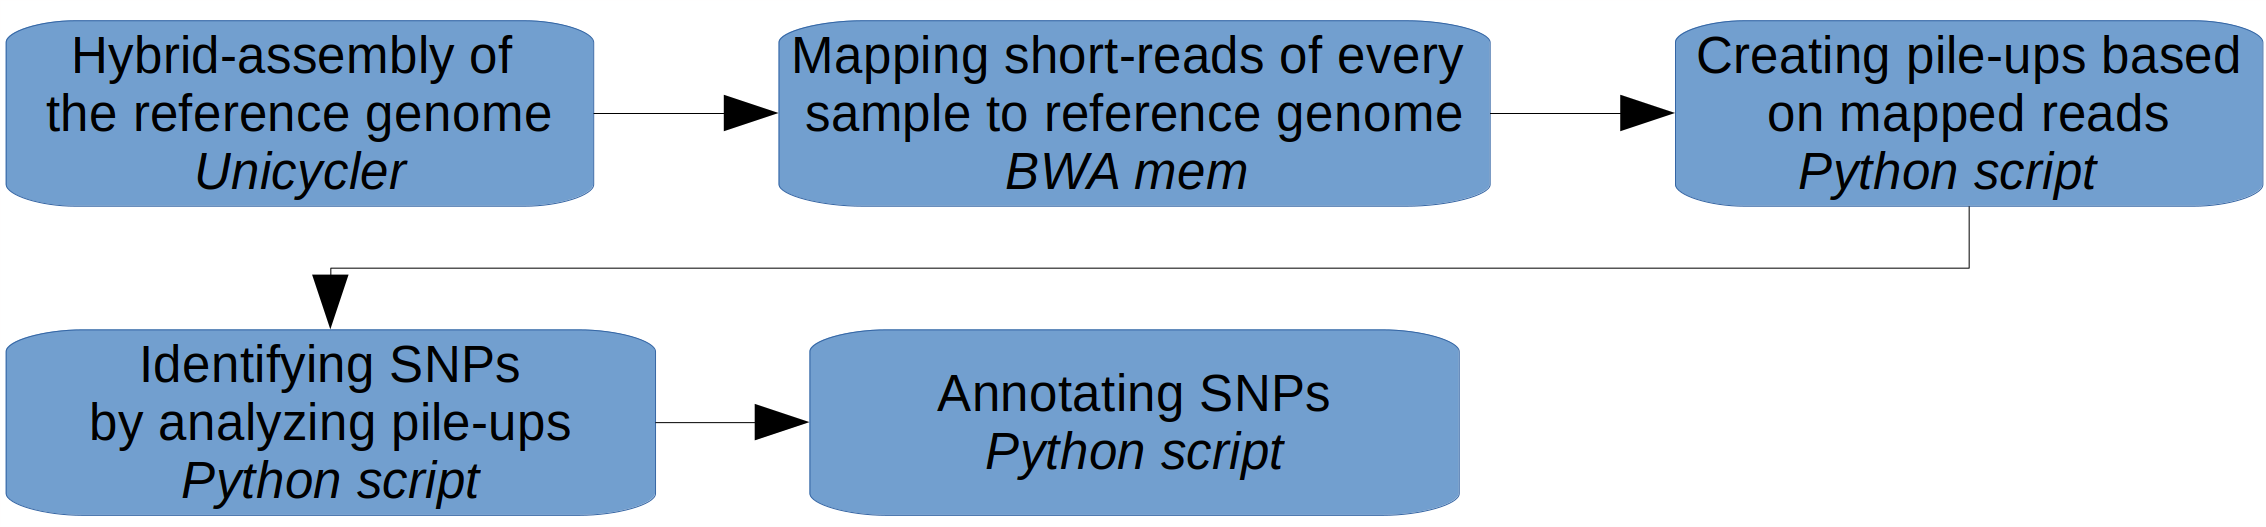
\includegraphics[width=0.9\textwidth]{pipeline.png}
	\caption{Bioinformatic pipeline used for the identification of mutations and affected genes/promotors.}
	\label{figure:pipeline}
\end{figure}
We established a bioinformatic pipeline which allowed us to identify mutations which accumulated by evolutionary pathways while ESBL \textit{E. coli} strains changed their phenotype from susceptible to resistant to cefepime. Thise pipeline was based on sequencing data coming from multiple samples which were taken while resistance evolved. Samples taken along such a pathway are also referred as sample series. The steps of the pipeline are shown in Figure \ref{figure:pipeline}.

\subsection{Creating a reference genome with annotation} 
The first step was to de novo assemble the genome of the sample with the lowest cefepime MIC of a sample series. We called the whole-genome assembly of this sample reference genome. For whole-genome assembling we used Unicycler \cite{wick_unicycler:_2017} as an assembler. With Unicycler \cite{wick_unicycler:_2017} we combined long-read sequencing data produced with Oxford Nanopore Technologies (ONT) and short-read Illumina sequencing into a hybrid-assembly. ONT sequencing was done by ourselves, Illumina sequencing by our collaborators of the University Hospital of Basel.  

\subsubsection{ONT sequencing}
For ONT sequencing the library was prepared with a ligation sequencing kit (LSK-108) followed with the native barcoding expansion kit. This allowed barcoding of multiple samples and loading all of them on a single flow cell (FLO-MIN106D). As a sequencing device we used the MinION from ONT. \\
As a fist step each DNA isolate was diluted to a concentration of 1 \textmu g/\textmu l in 50 \textmu L nuclease free water (NFW). For end-repairing the DNA 7 \textmu L NEBnext Ultra II Endrepair/dA-tailing enzyme mix were added to each
sample and incubated at 20\degree C for 5 min and at 65\degree C also for 5 min. After this step every sample was cleaned up by adding 60 \textmu of AMPure XP beads. The beads were incubated with the samples for 5 miuntes ona a rotor and then removed on a magnetic rack. Every sample was washed with 200 \textmu L 70\% ethanol which was repeated once. The ethanol was removed and every sample was suspended in 25 \textmu L NFW. 2.5 \textmu L of each barcode plus 25 \textmu L of Blunt/TA ligase was added to each sample and incubated for 10 minutes. All the samples were pooled and 500 \textmu of AMPure XP beads were added. After incubating the pooled sample for 5 minutes on the rotor the sample was washed again twice with 70 \% ethanol. All the DNA was eluted in 51 \textmu L NFW. The final sample was diluted to a concentration of 35 ng/\textmu L. Then for adapter ligation 20 \textmu L BAM, 30 \textmu L Ultra II ligation master mix and 1 \textmu L enhancer were added. After 10 minutes of incubation, 40 \textmu L AMpure XP beads were added and incubated on the rotor for 5 minutes. The supernatant was removed on the magnetic rack and the DNA was washed twice with ABB. The DNA was eluted and incubated for 10 minutes in 15 \textmu L ELB. Finally the library was prepared by mixing 15 \textmu L of eluted DNA in ELB with 25.5 \textmu L LLB and 35 \textmu L RBF. The resulting library was loaded on the flow cell, which was primed before with a mixture of 480 \textmu L RBF  and 520 \textmu L of NFW. The sequencing run was started and simultaneously base-called with Albacore.

\subsubsection{Illumina sequencing}
The DNA from the samples was isolated using the EZ1 DNA tissue kit on an EZ1 Advanced XL robotic system (Qiagen). The library for the sequencing was prepared using the Nextera XT library preparatino kit (Illumina) and the resulting library was sequenced on a MiSeq Illumina platform \cite{nanopore}. The reads produced with Illumina were trimmed with Trim Galore \cite{noauthor_babraham_nodate}.
\label{section:illumina}

\subsubsection{Annotating the reference genome}
Every reference genome was annotated with prokka (v.1.12) which produced a genbank file for every reference genome \cite{seemann_prokka:_2014}. Prokka first searches a core set of well characterized protein using BLAST+ and then compares reading frames to a database derived from UniProtKB \cite{seemann_:zap:_2019}. Additionally promotor regions were identifed using the promoter prediction tool PePPER \cite{pepper}. PePPER is a tool which takes whole-genomes as an input and predicts promotor sequences. Those sequences were mapped against the reference genome using graphmap \cite{sovic_fast_2016}. Furthermore a promotor data base hosted on EcoCyc was used. This data base contains around 3800 experimentally validated promotors for \textit{E. coli}\cite{noauthor_smarttable_nodate}. The sequences from this database were downloaded and mapped against the reference genome with graphmap aswell \cite{sovic_fast_2016}. 
\label{section:annotatiion_ref}

\subsection{Mapping Illumina sequencing data of the sample series to the reference genome}
As a second step of the pipeline the short-read Illumina sequencing data of every sample was mapped against the reference genome of the sample series. Mapping to the reference genome was done with BEW mem \cite{li_fast_2009}. This resulted in a bam file for every sample of the series. Mapping all the Illumina reads provided us the inofrmation which base was present in every Illumina read mapped to a certain position to the reference genome. If the most abundant base of all Illumina reads at a certain position is different than in the reference genome a mutation was present. To make this information more accessible we calculated pile-ups as a third step of our analysis. 

\subsection{Calculating pile-ups}
Pile-ups are count matrices which store which base is present how many times at a certain position considering every mapped Illumina read. In order to produce those pile-ups we used a script called \href{https://github.com/nahanoo/ESBL\_project/pileup.py}{pileup.py}. This script extracted the base counts by going through every position of the bam-file from a sample. Pile-ups were calculated for every sample of a series and all the pile-ups stored in a matrix stack. Next to identification of the most abundant base, pile-ups also allowed us to easily calculate base frequencies and the coverage which was easily comparable within a series because all pile-ups were stored in a matrix stack.

\subsection{Identification of mutations} 
We identified mutations by comparing the most abundant base at every position of the matrix-stack with a script called \href{https://github.com/nahanoo/ESBL\_project/pileup.py}{analysis\_modular.py}. If the most abundant base varied between the samples of the matrix-stack a single-nucleotide polymorphism (SNP) was identified. For the rest of the pipeline only mutations were included where the coverage was at least 30 and the base frequency at least 0.8.

\subsection{Identifying genes and promotors affected by mutations}
As a last step of the pipeline we checked if annotation was available for every found mutation. As described in section \ref{section:annotatiion_ref} genes and promoters were identified for every reference genome. \\
For checking if a SNP affected a gene, we analyzed the genbank file with biopython \cite{cock_biopython:_2009}. We checked if a mutation was located between a start and an end position of a gene. For checking if a SNP affected a promotor region we analyzed the bam-files which were created with the promoter sequences coming from PePPER and EcoCyc (see \ref{section:annotatiion_ref}). We checked if a SNP was loacted between a start or end positon of a mapped promotor sequence. 

\section{Analyzing ESBL \textit{E. coli} samples from patients at the University Hospital of Basel}
Our collaborators from the clinical microbiology of the University hospital of Basel collected 65 \textit{E. coli} samples of 34 patients. Those collected samples were all screened positive for ESBL genes. This resulted in ESBL \textit{E. coli} sample series with one to four samples per patient. The sampling period was between 2011 and 2015. Sample collection for one patient typically happened within several months.
\label{section:sample_collection}
\subsubsection{Screening for ESBL genes}
Coming after meeting with Adrian
\subsection{Selection of samples suitable for our analysis}
Our collaborators determined the MICs of every sample for the third-generation cephalosporin ceftazidim and the fourth-generation cephalosporin cefepim. Some sample series showed a significant change of the MICs. Sometimes resistance was gained, but in certain cases resistance was also lost. We were interested in identifying mutations in sample series where susceptibility significantly changed and all the samples from a series were the same ESBL \textit{E. coli} strain.
\subsubsection{Determination of the minimal inhibitory concentration}
Coming after meeting with Adrian.

\subsection{Pylogenetic analysis}
We checked if samples of a series were all the same ESBL \textit{E. coli} strain by running a phylogenetic analysis with Illumina sequencing data from the samples. For the phylogenic analysis we used a tool called PanX \cite{ding_panx:_2018}. Illumina data for every sample was provided by our collaborator (see Section \ref{section:illumina}) .

\subsubsection{PanX}
PanX is a tool which clusters samples based on their genes into orthologous clusters. From those clusters, panX identifies the core genome which are genes shared by all samples in the cluster. Based on those core genomes a strain-level phylogeny can be build, making use of single nucleotide polymorph positions (SNPs) within the core genomes. \\ 
PanX used annotated whole-genomes as input files that is why every sample was short-read assembled and annotated. For short-read assembling we used spades (v3.12.0) \cite{nurk_assembling_2013}, for annotating the resulting assemblies we used prokka (v.1.12) \cite{seemann_prokka:_2014}. The results from prokka were stored in a genbank file for every isolate. Based on those genbank files the PanX analysis was performed. \\

\subsection{Identification of mutations}
The selected sample series were analyzed with the pipeline described in \ref{section:pipeline}. For ONT sequencing the DNA was extracted  using the EZ1 DNA tissue kit on an EZ1 Advanced XL robotic system (Qiagen).

\subsection{Studying copy numbers of ESBL genes}
Next to hybrid-assembling the sample of a sample series with the lowest MIC we also hybrid-assemblied the rest of the samples using Unicycler \cite{wick_unicycler:_2017} ONT and Illumina sequencing data. The resulting assemblies were annotated with prokka \cite{seemann_prokka:_2014}. We did that because we were interested to see if the copy number of ESBL genes changed while resistance evolved. We also checked if the coverage of Illumina reads mapped to ESBL genes increased when we mapped Illumina data of the resistant sample of a series to the reference genome of the series.

\section{Assembling and handling procedure of the morbidostat}
The following system is an adapted version of Topraks built differing mainly in its pump system, controlling unit and software. Hardware which was not commercially available was built by the in-house mechanic and electronic workshop.

\begin{figure}
	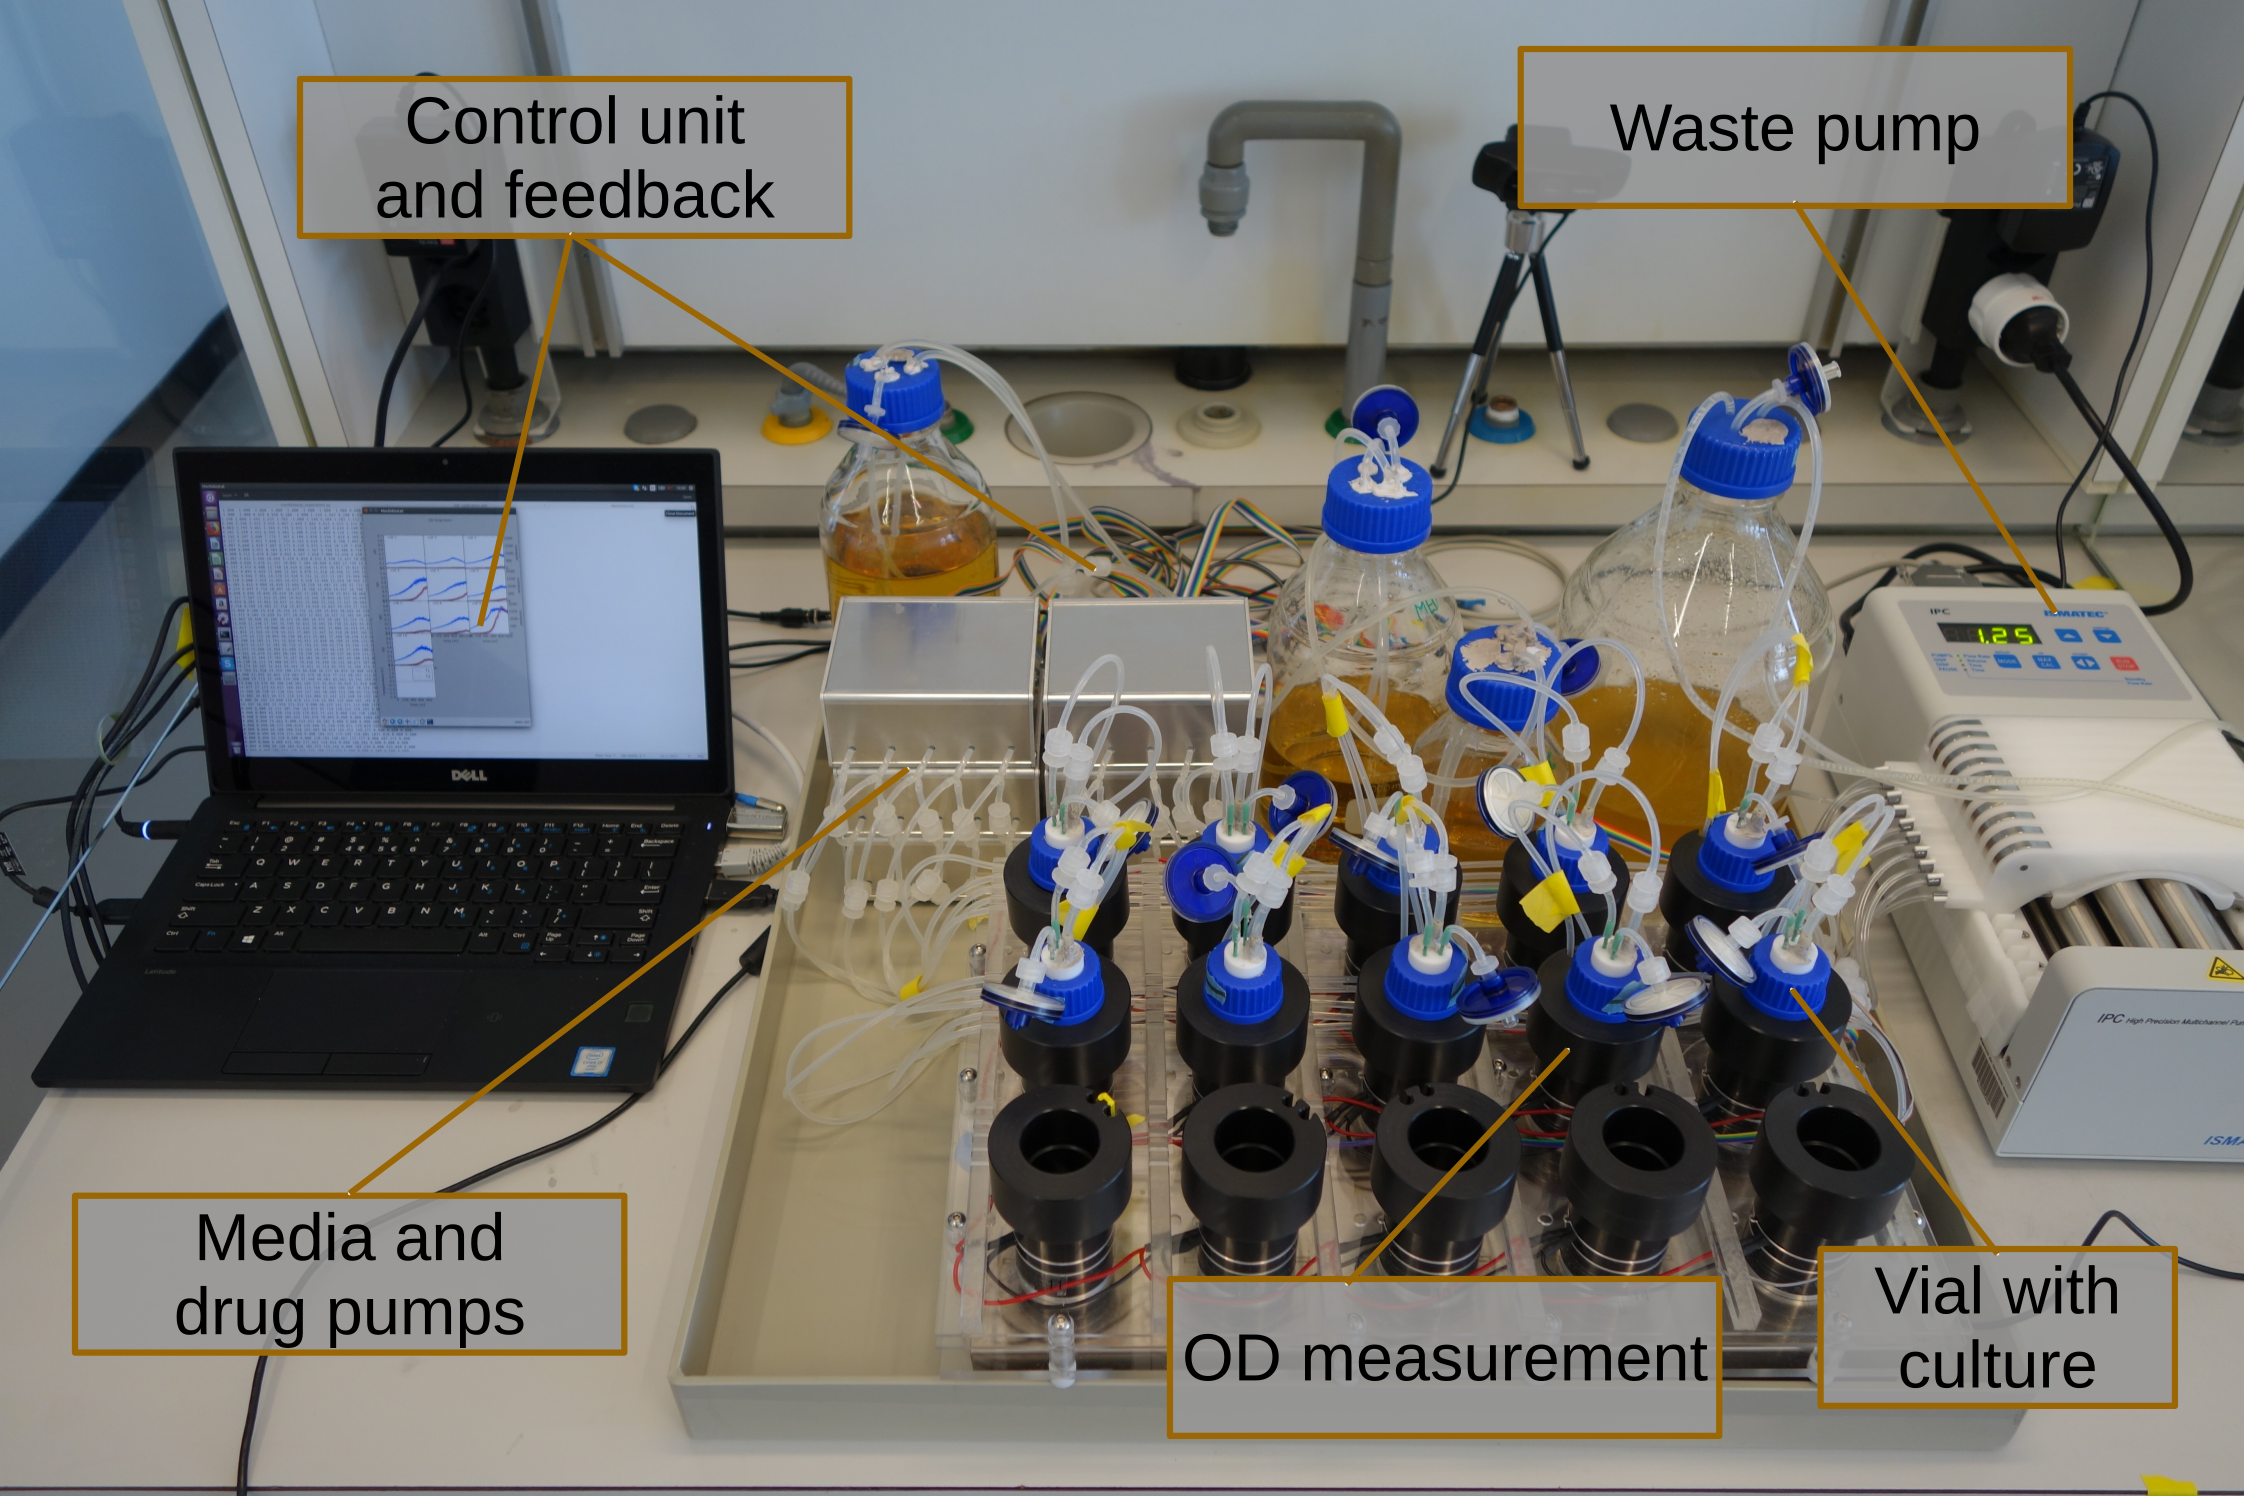
\includegraphics[width=0.7\textwidth]{setup_annotated_inksacpe.png}
	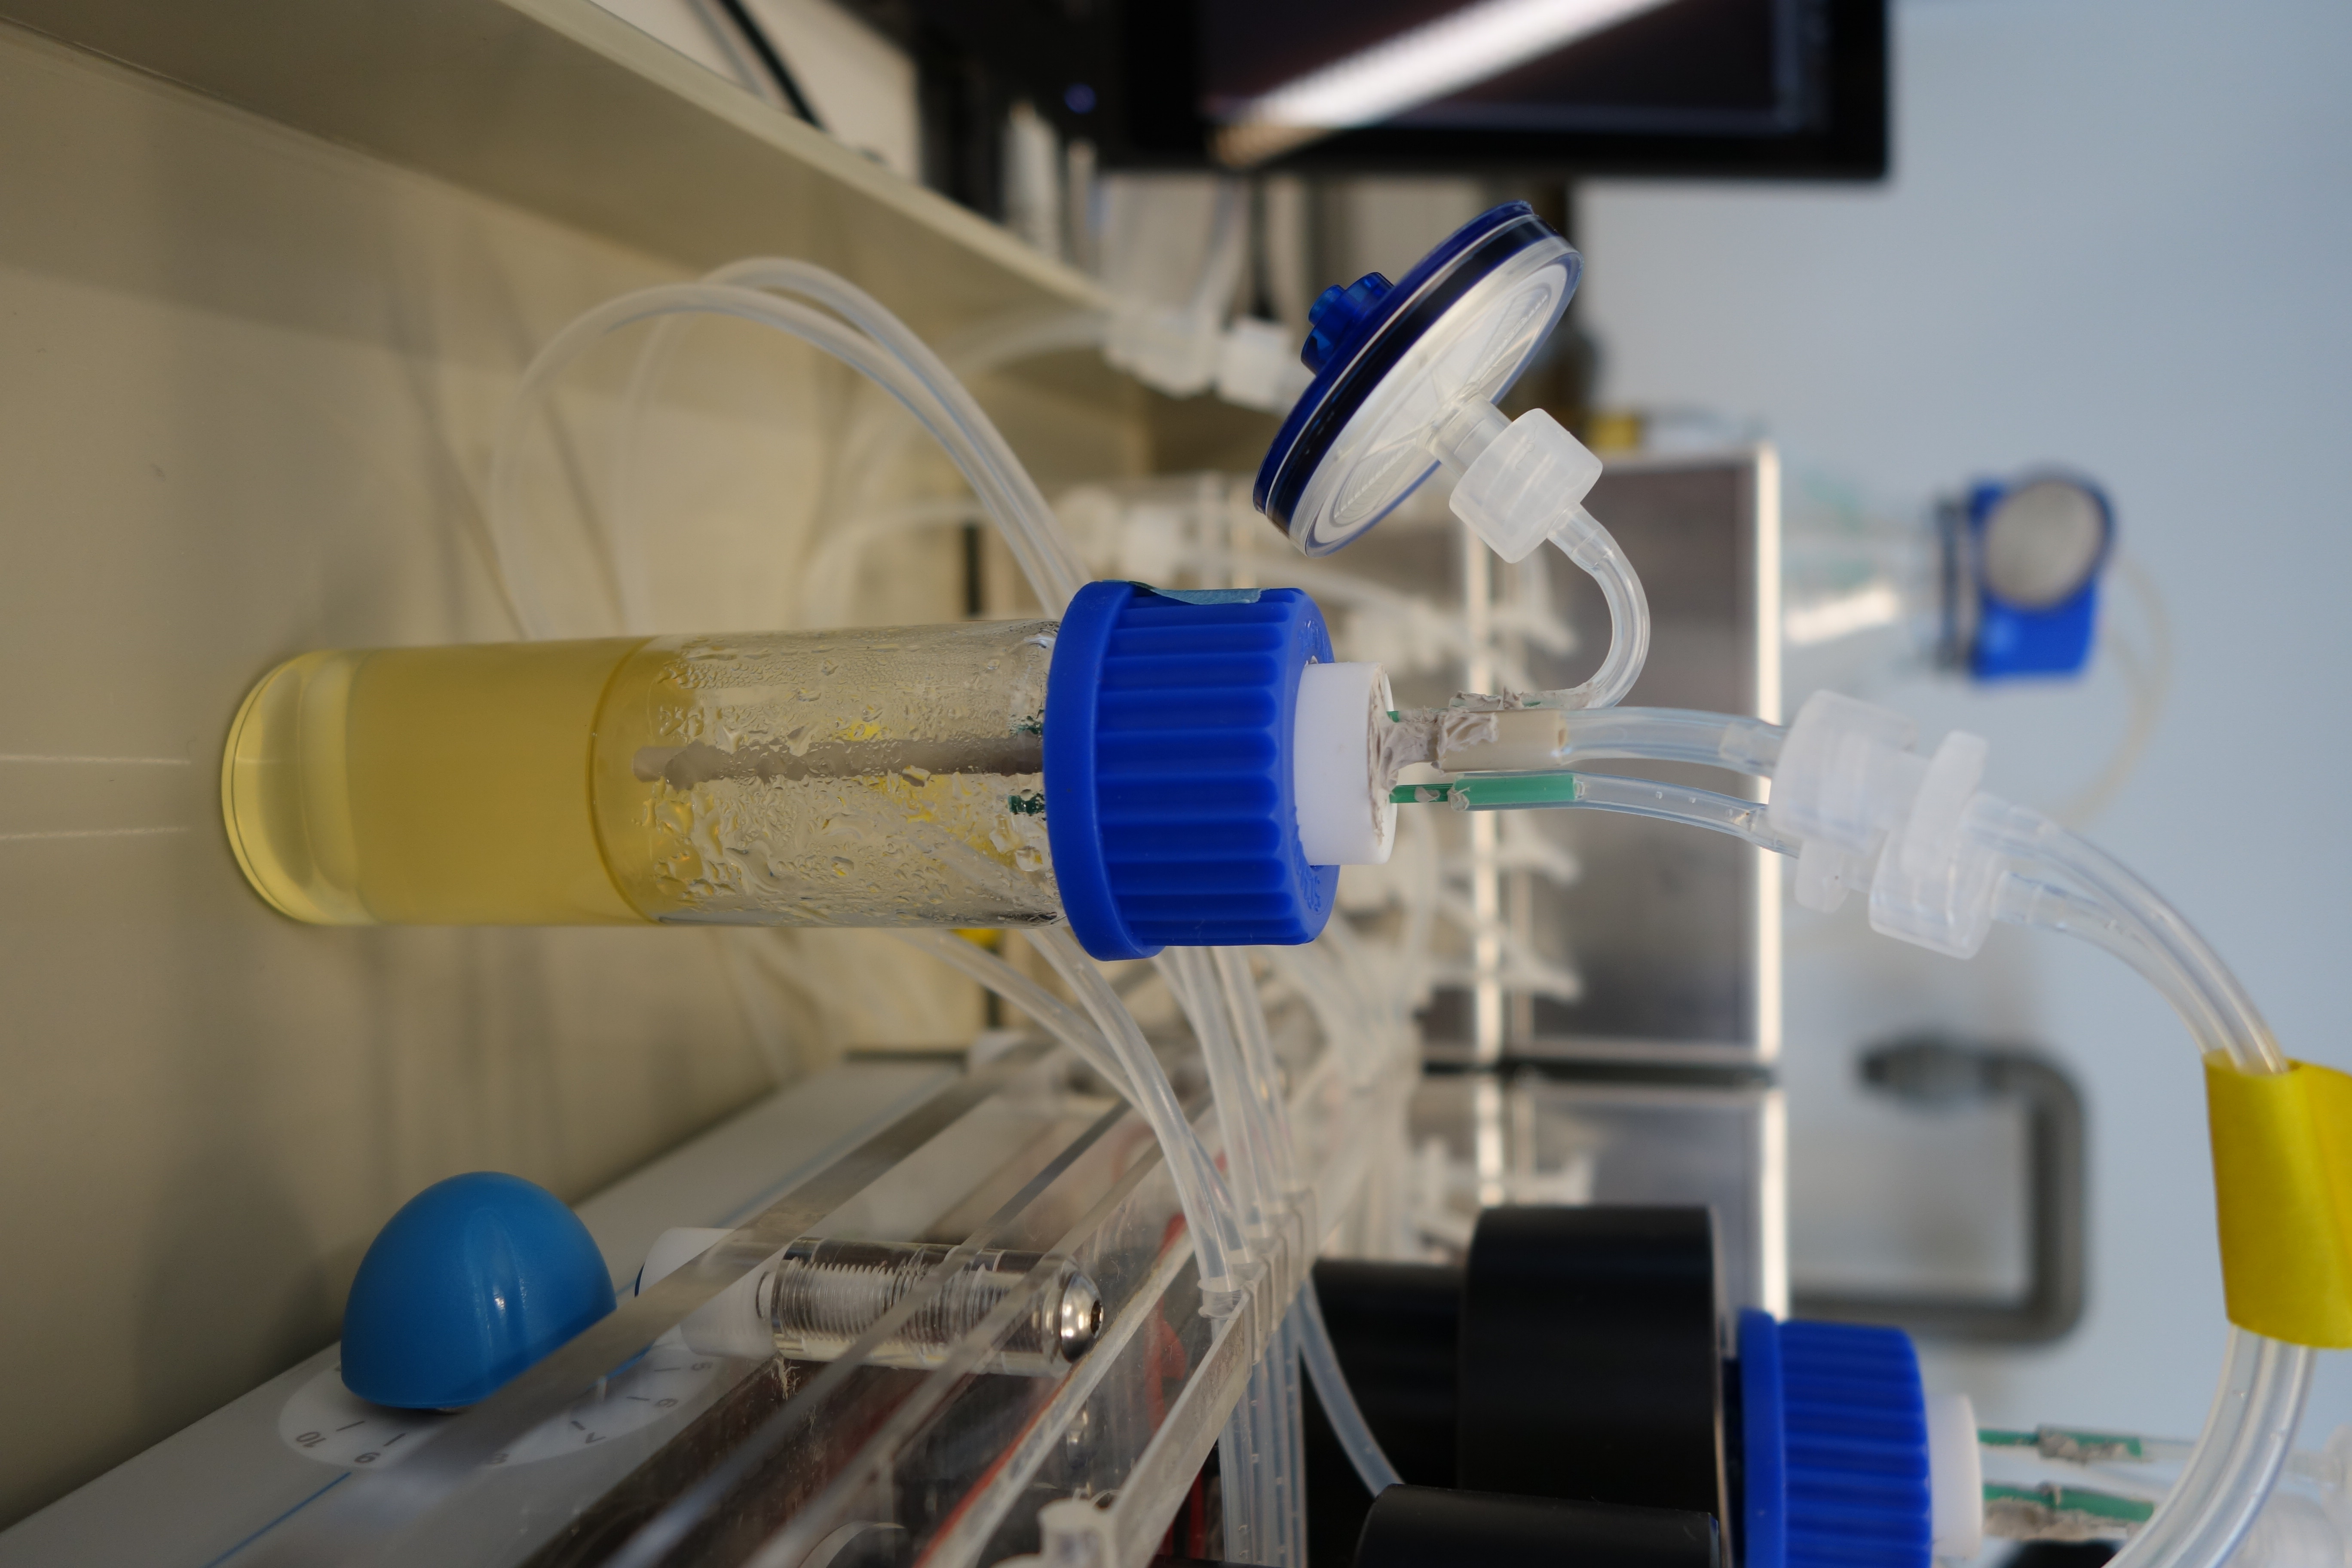
\includegraphics[width=0.4\textwidth,angle=90]{vial.JPG}
	\caption{Left: Overview of the morbidostat setup. The microcontroller is located behind the drug and media pumps. Right: One vial with all the inlets.}
	\label{figure:morbidostat_setup}
\end{figure}  
The left figure \ref{figure:morbidostat_setup} shows the morbidostat setup.
As a base for our built we used a magnetic stirrer with 15 slots. On that stirrer we placed three layers of acrylic glass through which we inserted black plastic rings which acted as our vial holders and optical density (OD) measuring units. 
The vials placed in the vial holders had three inlets as shown in the right Figure \ref{figure:morbidostat_setup}. One inlet was used to inject media or antibiotics, one for removing volume exceeding the culture volume and the last one to mount an air filter for pressure equilibration. \\
For Testing the hardware, we built the morbidostat in the open as shown in the Figure \ref{figure:morbidostat_setup}. For the actual experiments we placed the morbidostat inside a hypoxi-station in a bio safety lab 2. This allowed us to culture the bacteria at 37 \degree C but also to increase the safety. 


\subsection{OD measuring units}
For measuring the ODs was that we sent a ray of light through the cultures which was scattered by the cells. With the help of a phototransistor we could measure the scattering with analolg pins of the microcontroller. Because the scattering was proportional to the cell density, we could translate the scattering into an OD by calibration. \\
One OD measuring unit integrated in the vial holder is shown in  the right Figure \ref{figure:OD_unit}. Every unit consisted of a light emitting diode (LED) and a phototransistor. We chose OPB608A as a LED with a peak wavelength of 890 nm and PT 333-3C as a phototransistor, both from from TT electronics. For each unit the LED and the phototransistor were placed in a 135 \degree \space angle inside the vial holder. Both electronics were in direct contact with the glass vial.
The 15 OD measuring units were divided into three groups of five units which corresponds to one row of vials of the morbiostat. For every group the LEDs and phototransistors were both connected to independent 5 V circuits. The circuits of one group are illustrated in the left Figure \ref{figure:OD_cirguit}, where the LED circuit is shown orange and the photoransistor cicruict in blue. \\
The LEDs were constantly on sending rays of light through the cultures. When an OD measurement was initiallized the scattering was detected with the phototransistors. Light reaching the phototransistor caused an opening in the semiconductor from the phototransistor which led to an amplification of the current. This current reached a potentiometer connected in serial over which we measured the voltage with an analog pin of the microcontroller. The opening of the semiconductor altering the measured voltage correlated wih how much light reached it. More cells caused more scattering and more light reaching the semiconductor.\\
By measuring the voltages of differnet OD standards we calculated a linear equation describing the relationship between measured voltages and ODs.
\label{section:OD}
\begin{figure}
	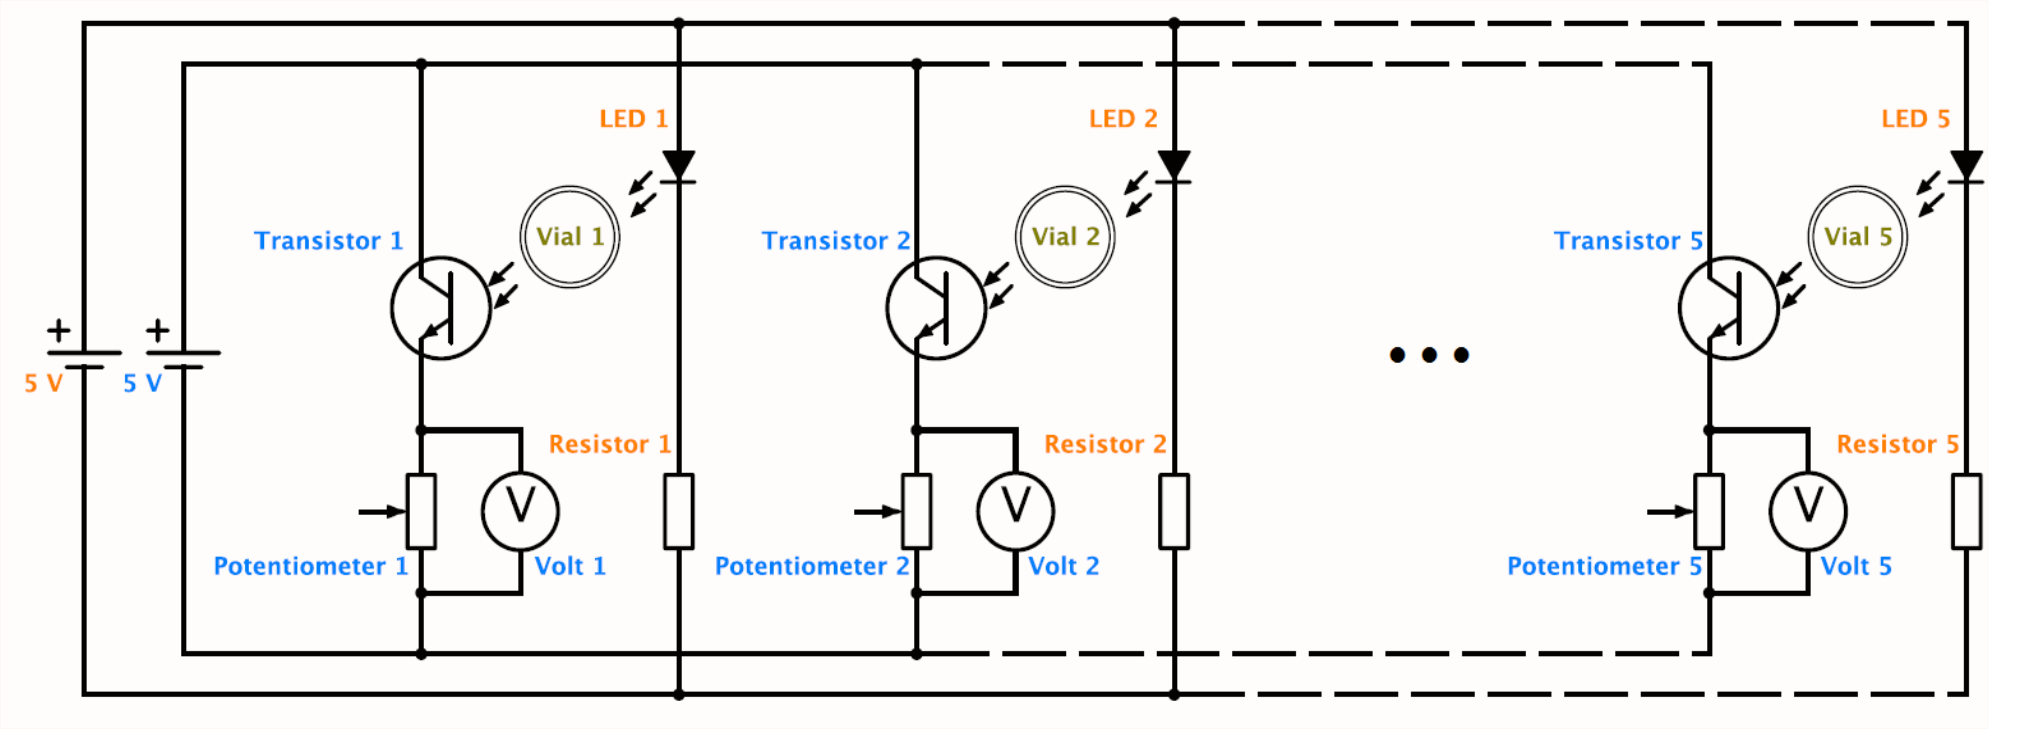
\includegraphics[width=0.6\textwidth]{OD_setup.png}
	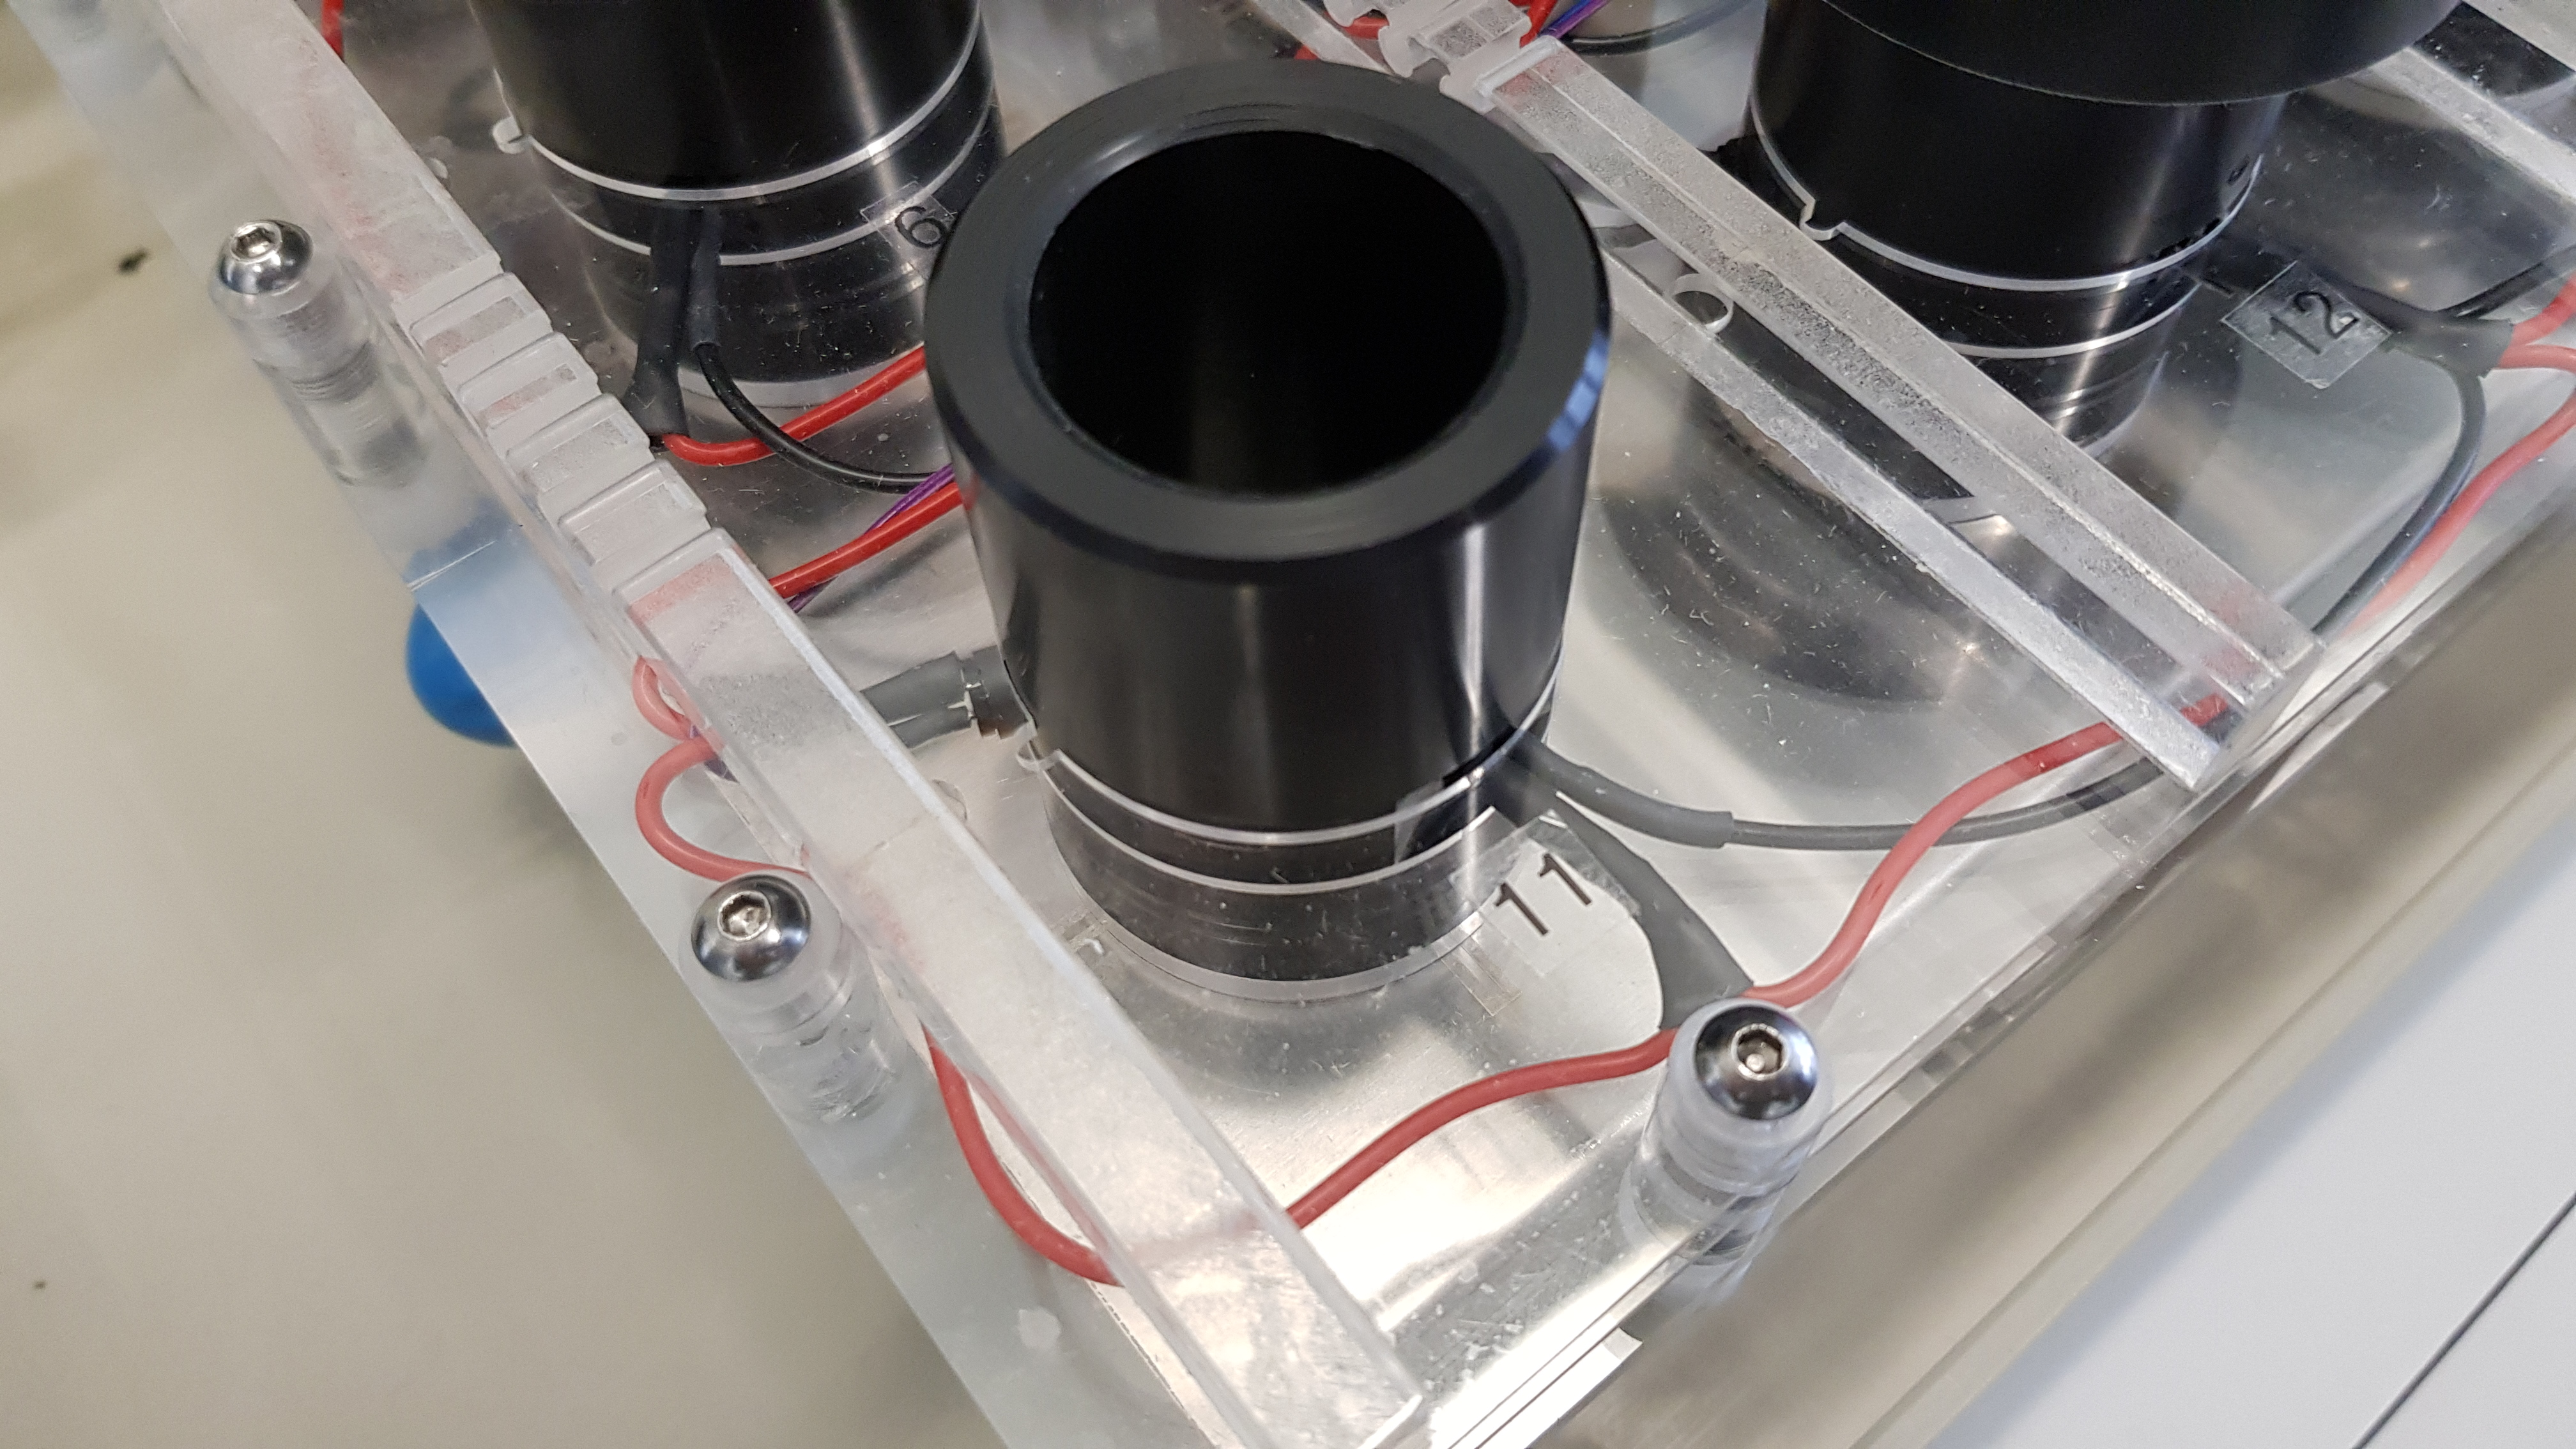
\includegraphics[width=0.3\textwidth]{OD_unit.png}
	\caption{Left: Circuit for parallel connected LEDs (orange). Each LED is connected in serial with a x \textOmega \space resistor. The circuit of the phototransistors is shown in blue. The phtototransistors are connceted in parallel. Each phototransistor is connected to a potentiometer in serial over which the voltage is measured with an analog pin of the microcontroller. Middle: Five mp6 pumps and their corresponding mp6-OEM controller mounted on the circuit board. Right: View on circuit board from below.}
	\label{figure:OD_cirguit}
	\label{figure:OD_unit}
\end{figure}

\subsection{Pumps and tubing} 
\begin{figure}
	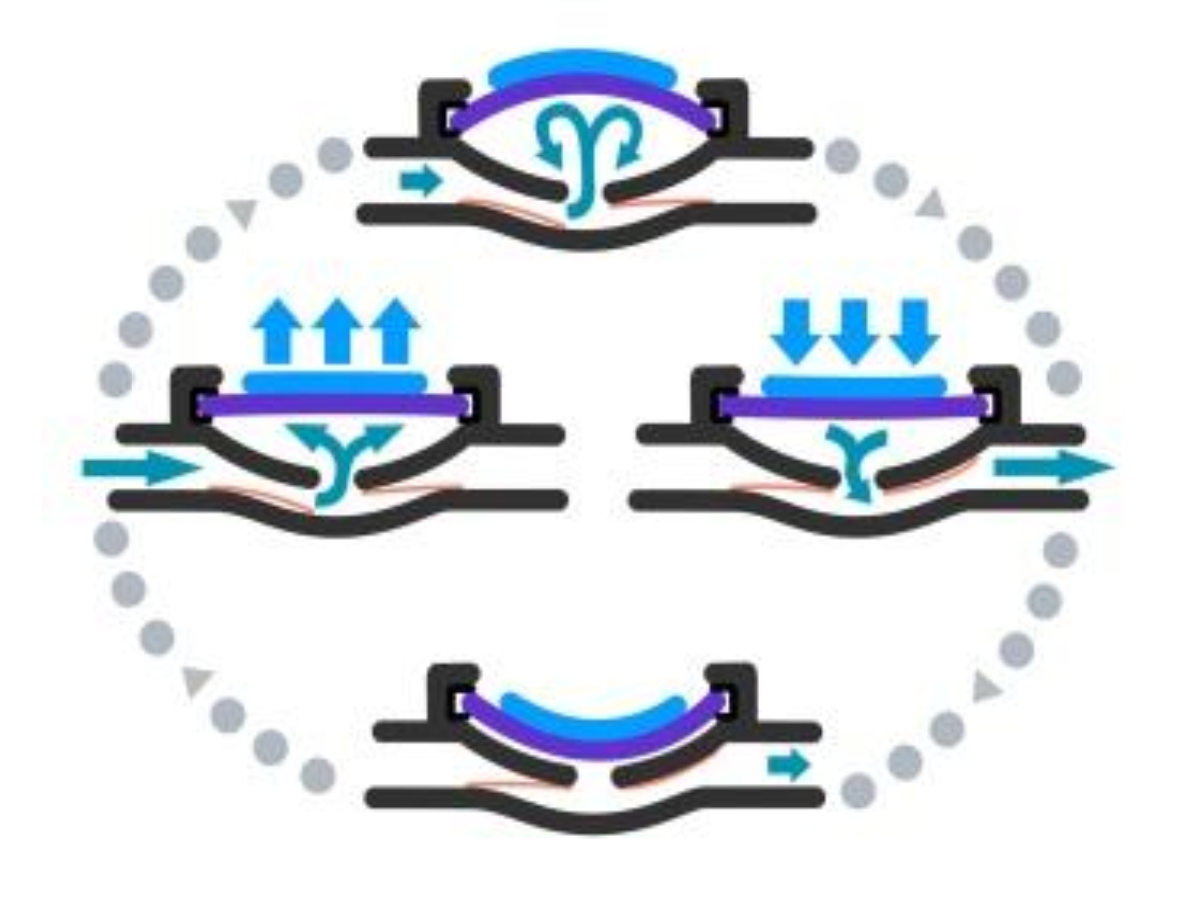
\includegraphics[width=0.2\textwidth]{piezo.png}
	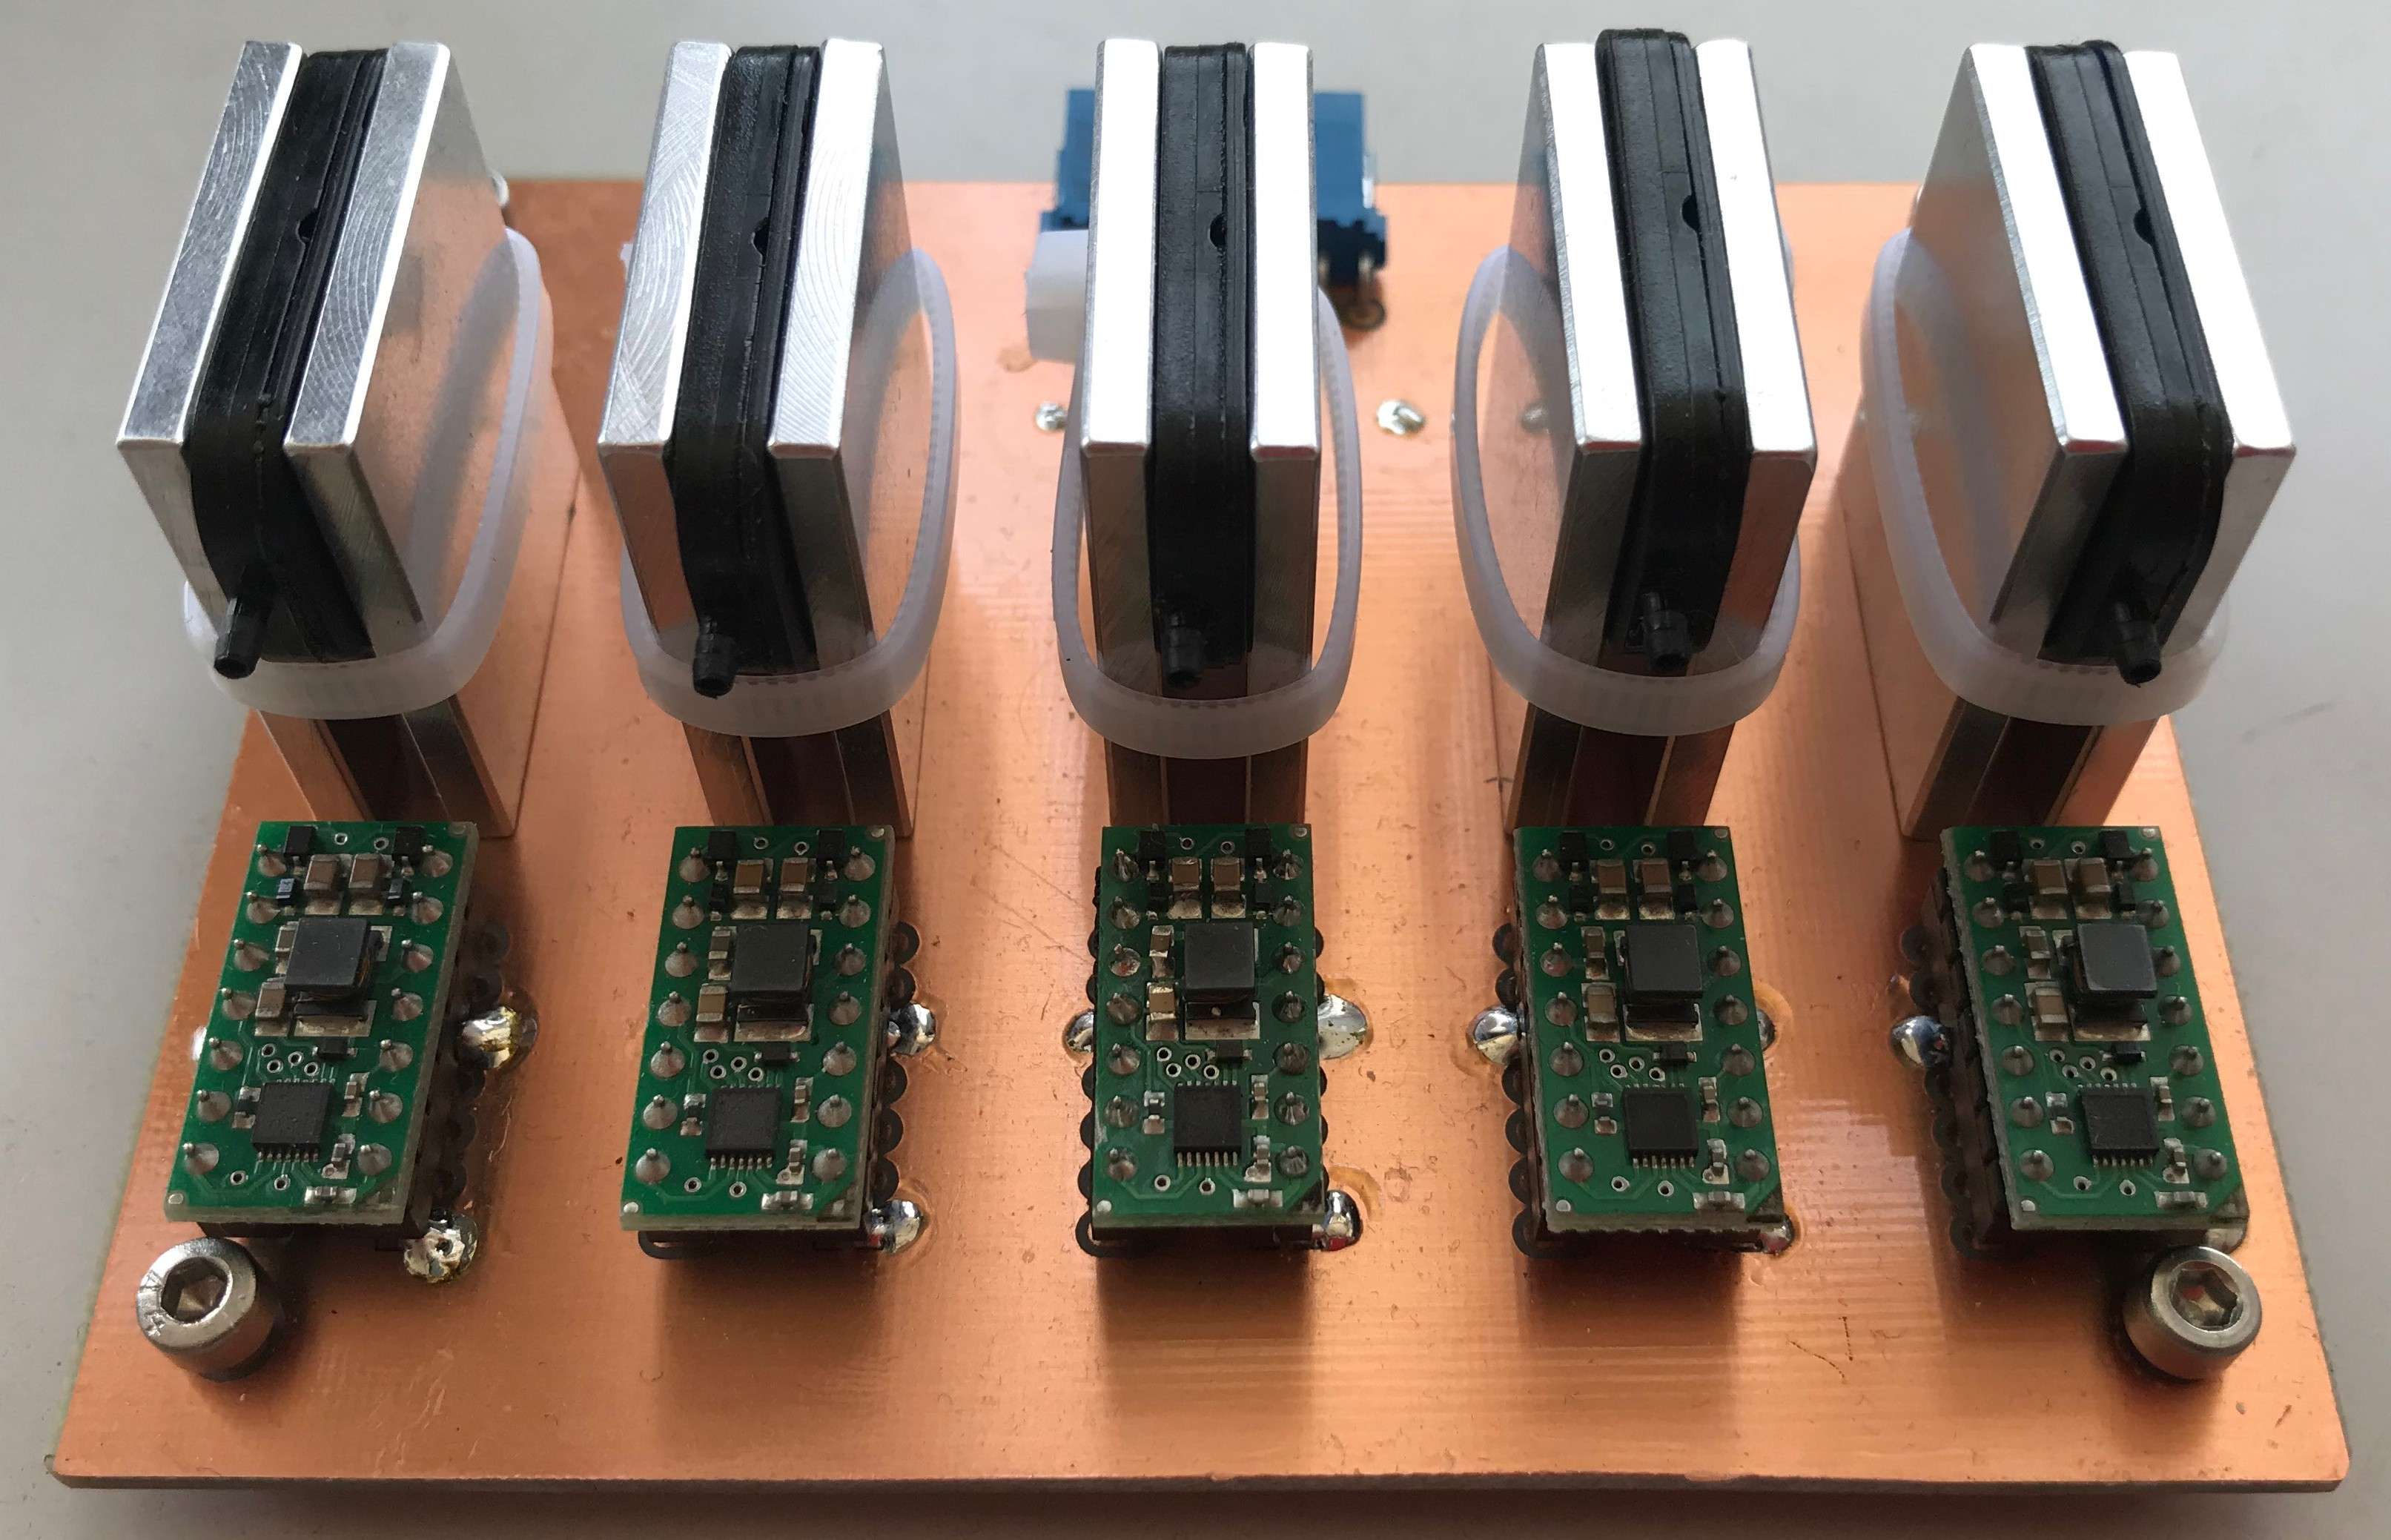
\includegraphics[width=0.4\textwidth]{board.JPG}
	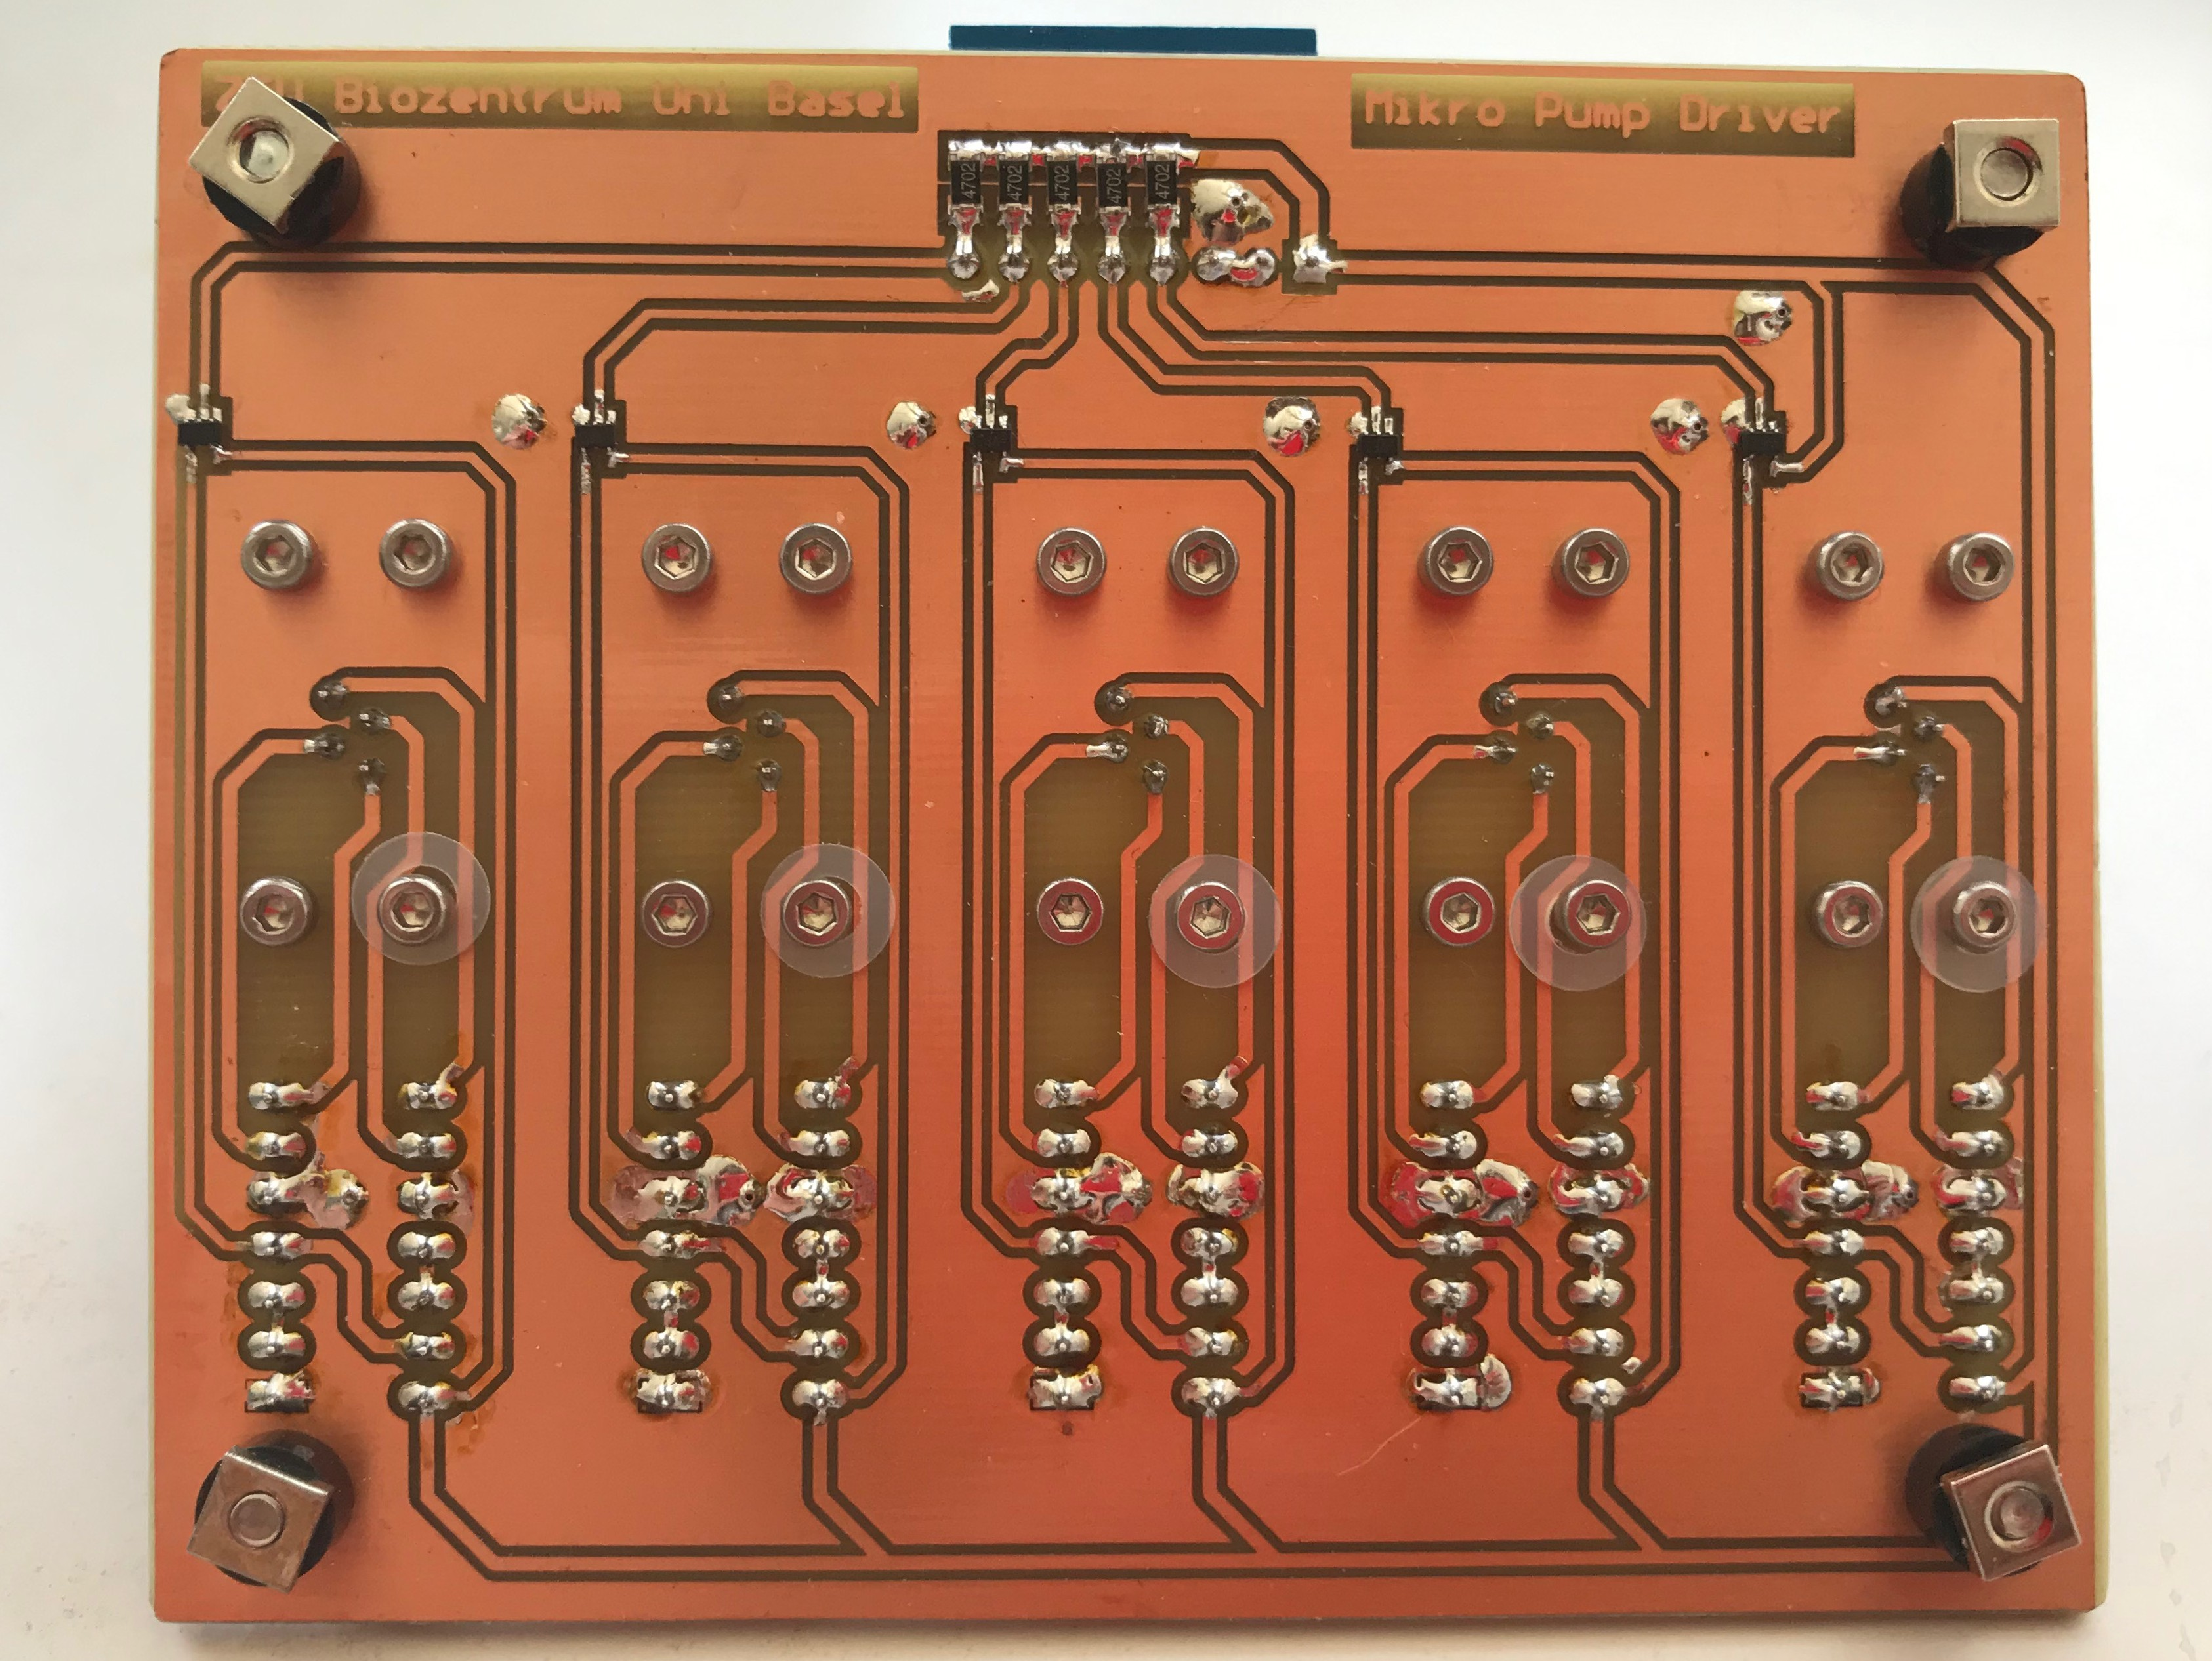
\includegraphics[width=0.4\textwidth]{board_below.png}
	\caption{Left: Principle of the pizo pumps. Top state: Piezo ceramic (purple) mounted on a membrane (blue) is relaxed.Left valve is open (orange), right valve  is closed, liquid enters. Right and bottom state: Voltage is applied to the piezo ceramic deforming the membrane resulting in a down stroke. Left valve is closed, right valve is open Liquid exits to the right. Voltage decreases again and the piezo ceramic enters its relaxed state again \cite{piezo_pumps}}
	\label{figure:pumps}
\end{figure}
\begin{figure}
	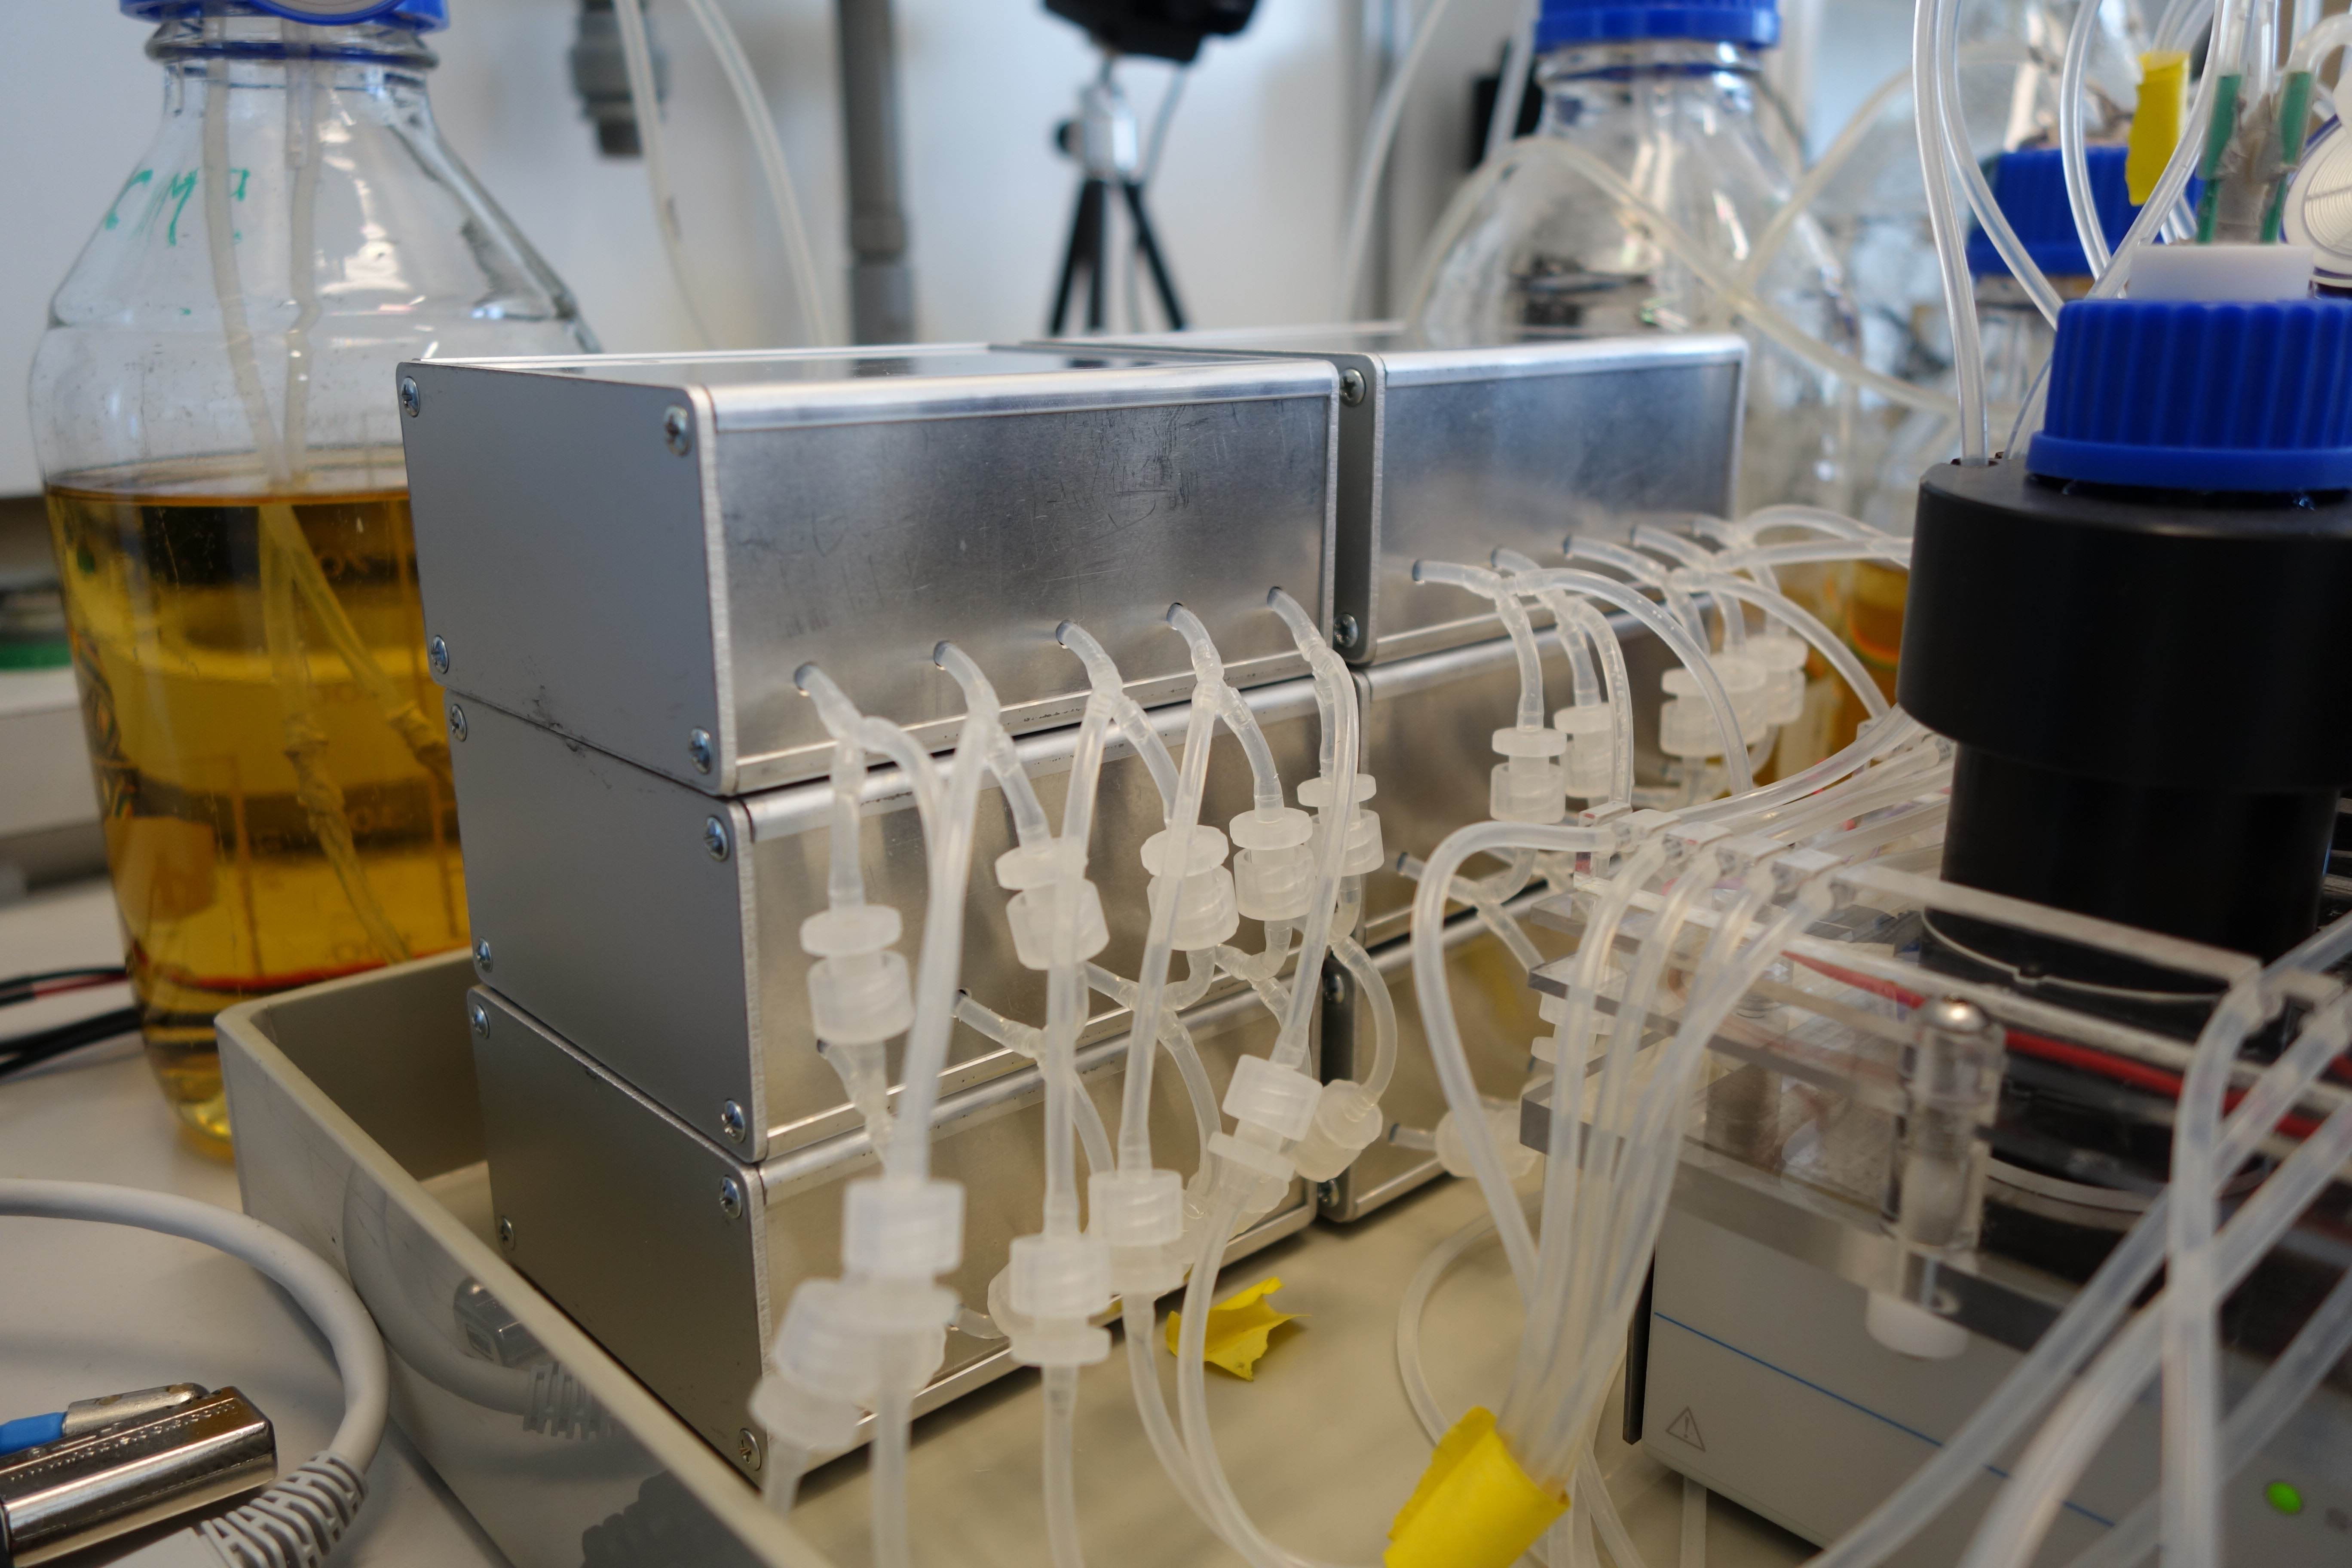
\includegraphics[width=0.5\textwidth]{pump_blocks.JPG}
	\caption{Figure left: Vial setup. Figure right: One row of five pumps represents one row of five vials. Since every vial is connected to three pumps, three rows of pumps are stacked on top of each other and connected column by column. This means that one column of three pumps is responsible for injection fluid into one vial. Every outlet from a pump from one column is connected, in order that there is just one tube going to one vial. }
	\label{figure:tubing_setup}
\end{figure}
Every vial was connected to three injecting pumps. One pump was responsible for injecting media, one for injection a low-concentrated antibiotic and one for injecting a high-concentrated antibiotic. Mixing of desired antibiotic concentration was possible by controlling the run times of the pumps.
We chose mp6 pumps from microComponents because of their very compact built. The functional principle of the pumps is shown in the left Figure \ref{figure:pumps}. We achieved a steady flow rate of the pumps with the the mp6-OEM controller from microComponents. On one circuit board five pumps with five mp6-OEM controllers were mounted which is shown in the middle Figure \ref{figure:pumps}. Each mp6-OEM controller was connected to one pump, a 5 V power supply, a ground and a digital pin of  the microcontroller which allowed computer controlling the run times of every pump. The circuit boards were mounted in a metal box and three of those boxes stacked on top of each other which is shown in Figure \ref{figure:tubing_setup}. Pumps of the lowest box were connected to media, pumps of the middle box to a low-concentrated antibiotic and the pumps of the top box to a high-concentrated antibiotic. We connected the outgoing tubes of the pumps from one stack column by column resulting in one outgoing tube per column as shown in Figure \ref{fiuger:tubing_setup}. Those tubes were led to the vials. This way we connected one vial with three pumps ranging all concentrations and leading just one tube to the vial.\\
Every vial was also connected to a 16-channel peristaltic pump which removed volume exceeding the culture volume through the grey tube show in the right Figure \ref{figure:morbidostat_setup}. 

\subsubsection{Computer controlling the pumps}
In order to control the run times of the pumps a pin of every mp6-OEM controller was conncected with a digital pin of the microcontroller. If the pin of the mp6-OEM controller received a voltage of 5 V the pumps were off, if the pin was set to ground the pumps were on. \\
When we set the digital pins of the microcontroller to ground there was still a low current flowing, resulting in a small voltage. The mp6-OEM controllers reacted very sensitive to this small voltage leading to weird behavior of the pumps. We solved this by inserting a pull-down resistor between the digital pins of the microcontroller and the ground which is shown in the right Figure \ref{figure:pumps}. Additionally an inverter was connected in serial to the digital pins. To turn on a pump the digital pins of the microcontroller was set to 5 V. The inverter connected in serial caused that the pin of the mp6-OEM controller was set to ground and the pumps were turned on. Run time control was possible by setting the digital pins to 5 V for the desired runtime.
The 16-channel peristaltic pumps was also computer controllable because the pumps was also connected to a digital pin of the microcontroller.
\label{section:pumps}

\subsection{Controlling the morbidostat}
As a microcontroller we used an Arduino mega 2560 flasehd with an arduino-script called \href{https://github.com/nahanoo/ESBL\_project/}{arduino\_interface.py}, which allowed us to change the state of digital pins or measuring voltages of analog pins. The microcontroller itself was controlled by a laptop where twho two python scripts were running. The python script \href{https://github.com/nahanoo/ESBL\_project/}{morbidostat\_experiment.py} decided which analog pins were measured and which digital pins were set to high for how long. Those tasks were grouped in cycles and repetitively executed. Additionally this script was responsible for storing ODs and injected antibiotic concentrations. We used a second pyton script called \href{https://github.com/nahanoo/ESBL\_project/}{arduino\_interface.py} to enable the communication between the laptop and the microcontroller. Commands for the microcontroller initialized by \href{https://github.com/nahanoo/ESBL\_project/}{morbidostat\_experiment.py} were encoded in a string by \href{https://github.com/nahanoo/ESBL\_project/}{arduino\_interface.py} which was transmitted to the microcontroller via a serial USB connection. The microcontroller interpreted the string and executed the encoded commands. \\
We implemented three modes for the morbidostat in \href{https://github.com/nahanoo/ESBL\_project/}{morbidostat\_experiment.py}. Those being the the continuous mode which we used for continuous inhibition of the cultures, a growth rate mode where growth rates with no injections were recorded and a fixed OD mode where the OD of a culture was fixed to a certain OD by dilution with media. \\   

\subsubsection{Tasks of a continuous morbidostat cycle}
As for every mode the continuous mode consisted of several tasks grouped in one cycle. Shown in Figure \ref{figure:flowchart} as a first step the microcontroller measured the voltages of the analog pins connected to OD measuring units for a defined cycle time (typically being 10 minutes). Those voltages were constantly send to the laptop where they were translated to ODs which were saved. After the cycle time a fit was calculated representing the OD measurements of a cycle for every vial. Using this fit the growth of every vial was calculated and stored. Additionally the measured ODs of a cycle where averaged and stored as well. Then a feedback algorithm calculated how much drug was injected into which vial. Shown in Figure \ref{figure:flowchart} the last step of a was to translate the calculated antibiotic concentration into run times of the three pumps connected to a vial. The run times were send to the microcontroller. The microcontroller turned on the pumps for the calculated time and after removing volume exceeding the culture volume with the peristaltic pump one cycle was finished. \\
The commandflow of the growth rate mode was very similir just that the feedback function was not executed and therefore no fluids were injected into the vials. For the fixed OD mode another function instead of the feedback  calculated how much media was injected in order that the OD was kept at a steady value. 
 
\begin{figure}
	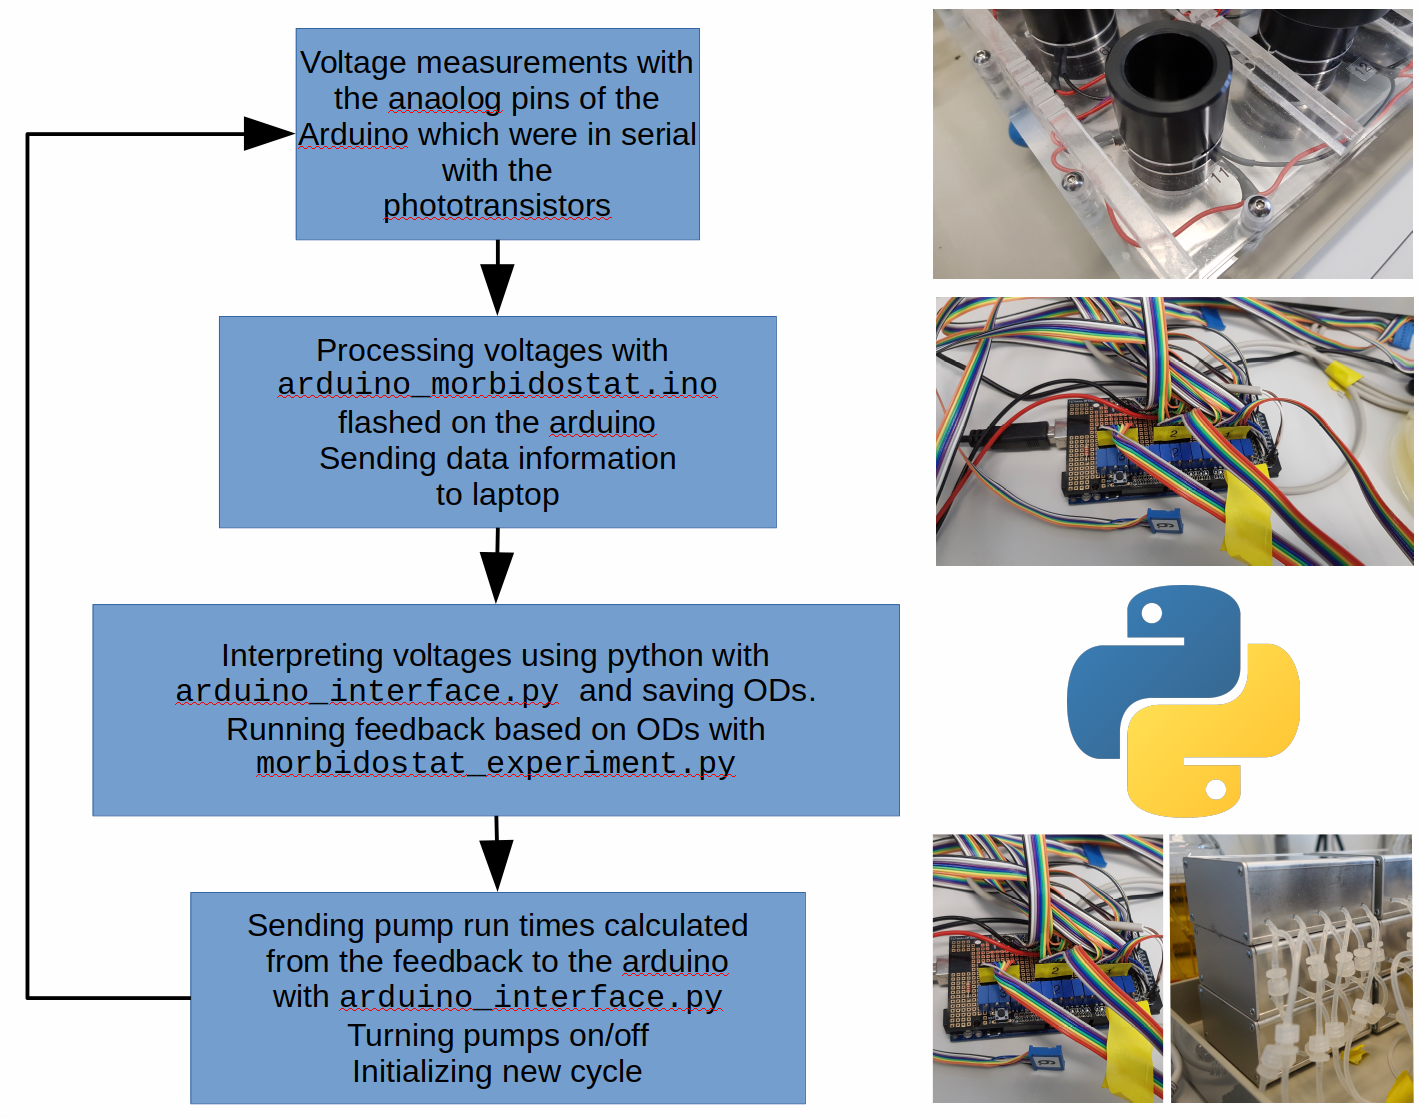
\includegraphics[scale=0.25]{flowchart.png}
	\caption{Overview of one cycle from the continuous mode of the morbidostat.}
	\label{figure:flowchart}	
\end{figure}

\subsubsection{Feedback of the continuous mode} 
The feedback determined how strongly the cultures were inhibited. This feedback was based on the relative difference between the averaged ODs of the current cycle and the averaged ODs of a past cycle. We called averaged ODs of a cycle final\_OD and the relative difference between two final\_ODs \textDelta OD. 
\begin{center}
	$\Delta OD = (final\_OD_{x_{cycles\_back}} - final\_OD_{current\_cycle})/x$
\end{center}
As shown in in Figure \ref{figure:feedback} the feedback did several comparisons before calculating an appropriate dose of antibiotics. As a first step it checked if \textDelta OD was positive or negative. A negative \textDelta OD implied that the bacteria were dying. In order to prevent complete sterilization, media was injected in this case. \\
When \textDelta OD was positive the bacteria were growing. Antibiotics were only injected if the bacteria reached a certain OD called drug\_dilution\_threshold. Therefore, the next comparison as visible in Figure \ref{figure:feedback}, was whether or not the final\_OD was higher or smaller than this threshold. If the final\_OD was smaller no fluids were injected.
However when final\_OD was bigger than the threshold calculation of the appropriate dose was initialized.
The calculation itself was split up into two equations. One equation, mainly important at the beginning of the morbidostat experiments, was used to approximate the MIC of the strains. This was done by simply adding a fraction of the MIC for every cycle. After the MIC was reached this equation was ignored and from now on the second equation determined the injected concentration. This equation multiplied the current drug concentration in the vials by the \textDelta OD which resulted in how much the drug concentration in the vial was increased.
The goal of the feedback was that a certain OD called target\_OD was approximated in every vial. In order to do so we divided the second equation by this target\_OD. Now if a small target\_OD was chosen the increased concentration was divided by a small value causing a higher injected concentration. If target\_OD was set to a high value the divided outcome was smaller. 

\begin{figure}
	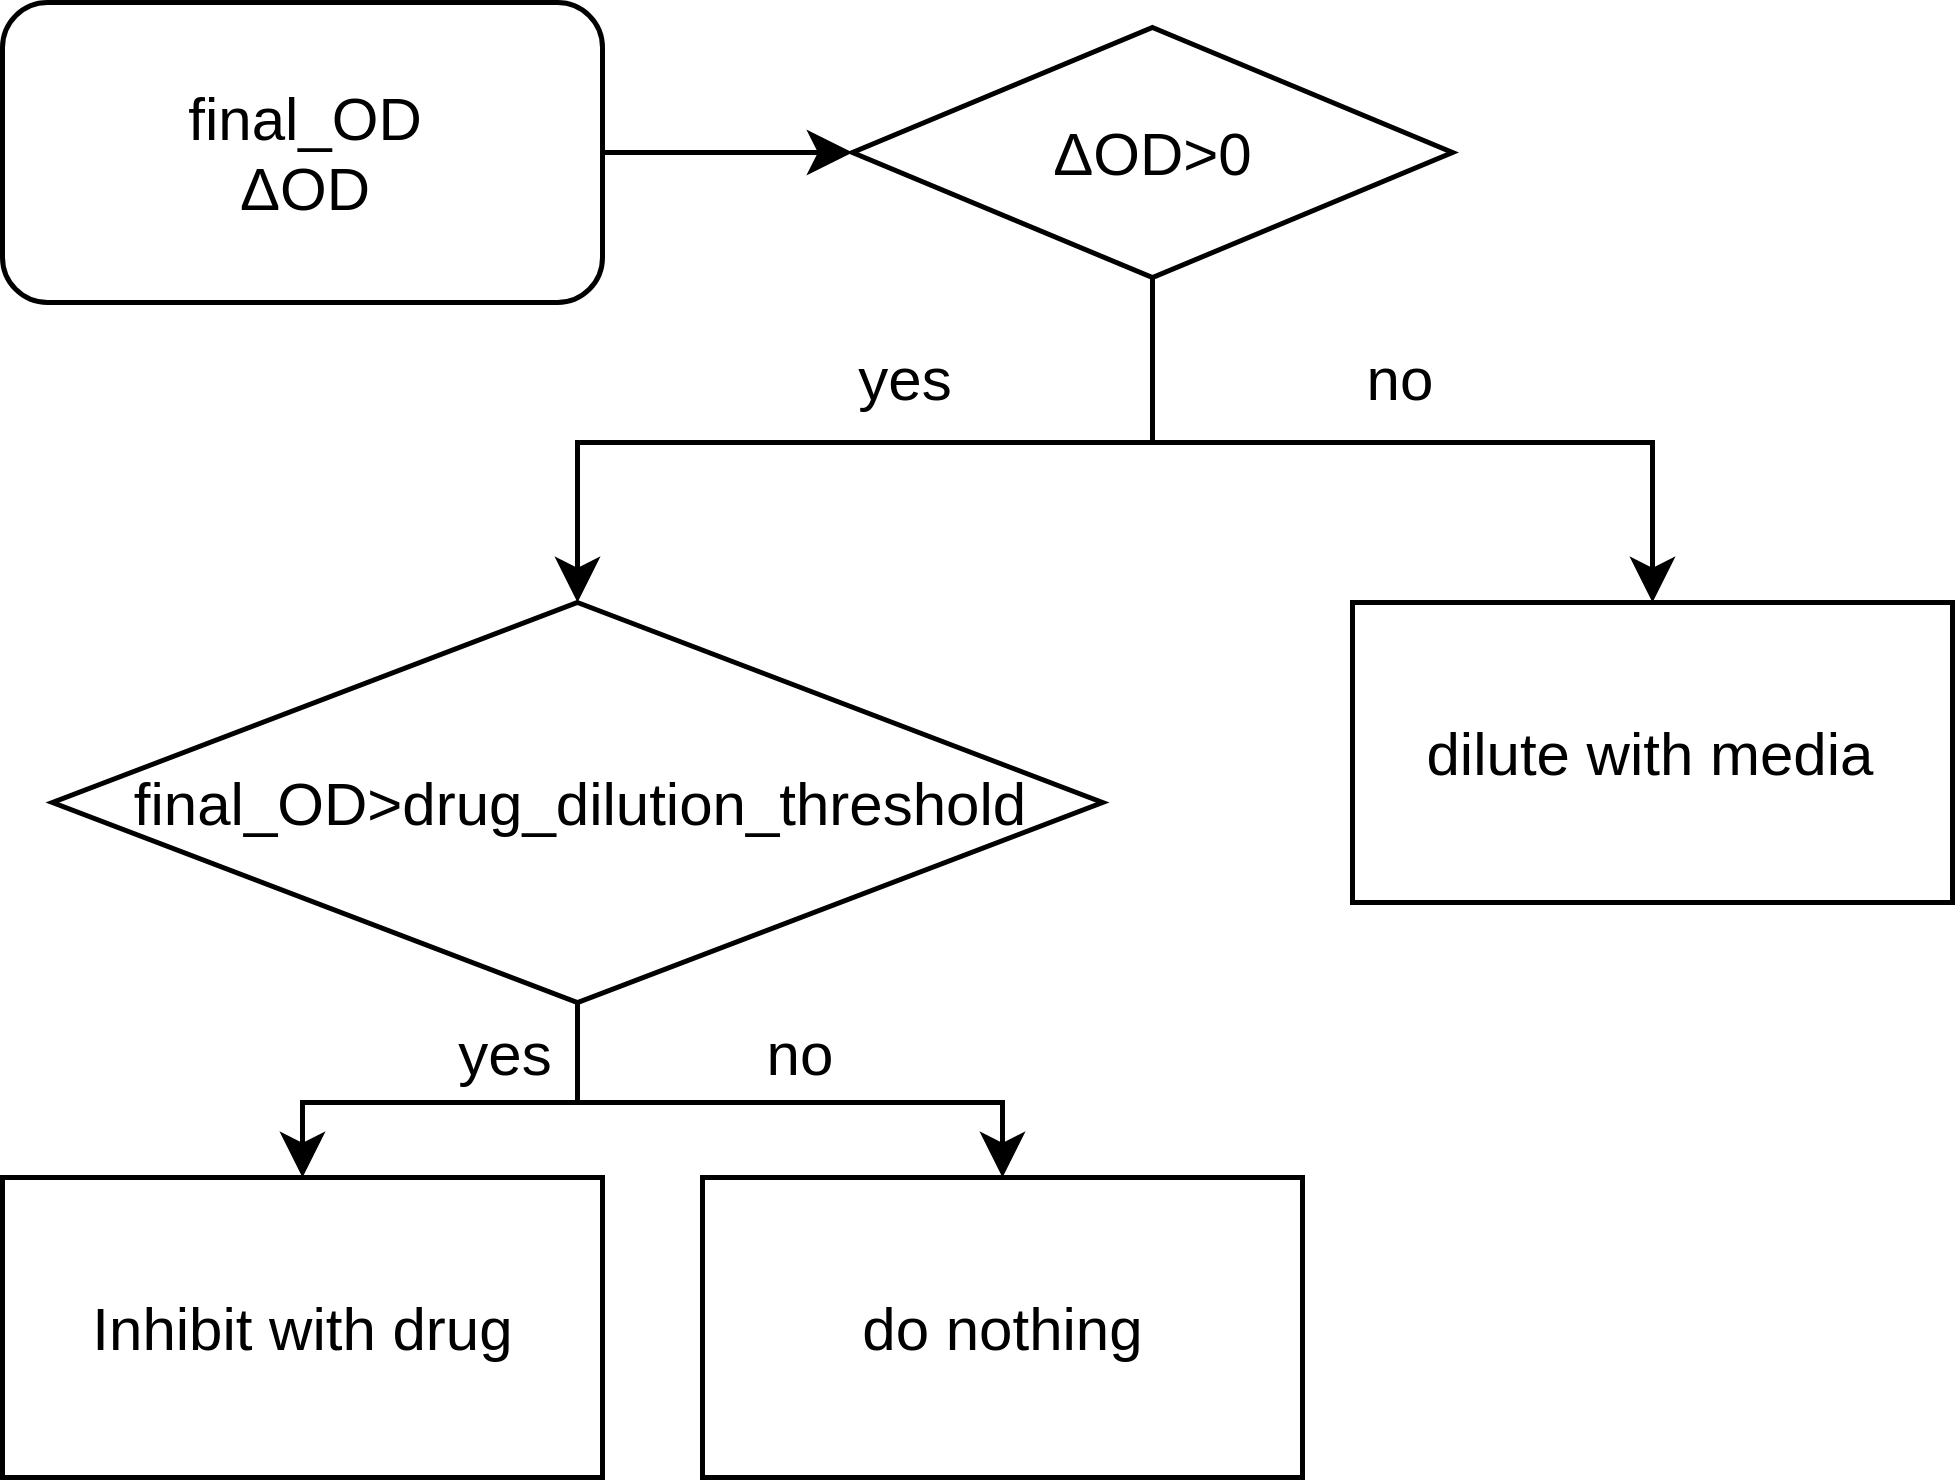
\includegraphics[scale=0.13]{feedback.png}
	\caption{Schematic overview of decisions involved in the feedback}
	\label{figure:feedback}
\end{figure}

\subsection{Hardware calibration}
\subsubsection{OD and pump calibration}
For calibrating the OD measurements an overnight culure with K12 XL1 blue E. coli was inoculated in 5 ml 9/10 $H_2O$ and 1/10 LB media (also referred as diluted media). The next day the overnight culture was diluted 1/200 in 50 ml diluted media. After a few hours of day culturing following OD standards were prepared with 18 ml diluted media in the vials for the morbidostat: 0.01 0.021 0.042 0.107 0.192 0.278\\
Then every vial with a certain OD was placed in every vial holder. With the function calibrate\_OD from the \href{https://github.com/nahanoo/ESBL\_project/}{morbidostat\_experiment.py}, a voltage measurement was done for every OD standard and every OD measuring unit. The result of this function was a linear equation which translated the voltages to ODs. \\
\begin{figure}
	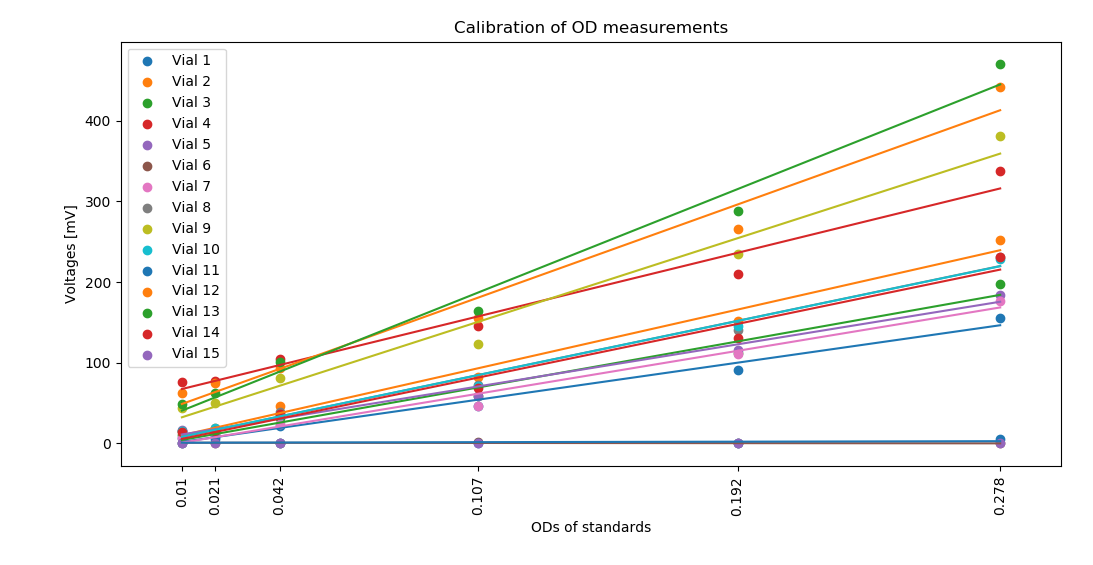
\includegraphics[width=1\textwidth]{od_calibration.png}
	\caption{Calibration of OD measuring units, with the OD standards on the x-axis and the measured voltages on the y-axis. The line represents the calculated linear equation. The units of vial 5 and 15 were not working.}
\end{figure}
For calibrating the pumps the function calibrate\_pumps from the\href{https://github.com/nahanoo/ESBL\_project/}{morbidostat\_experiment.py} was executed. The weight of every empty vial had to be entered and the function turned on every specified pump for 100 seconds. Afterwards the weight of the vials was entered again and the function calculated the flow rate for the specified pumps. 
\label{section:OD_calibration}

\section{Forcing cloned ESBL E. coli to evolve with the morbidostat}
\subsection{Producing ESBL E. coli clones}
Our collaborators produced three ESBL E. coli strains with gibson cloning. In order to do so the sequences of three ESBL genes and their upstream region were extraced from two samples of the sample collection described in \ref{section:sample_collection}. More coming soon, meeting scheduled with Bea this Friday.  

\begin{table}[H]
	\begin{tabular}{|c c|}	
		\hline
		Plasmid ID & ESBL \\
		\hline
		pEU22 & CTX-M-1 \\
		\hline
		pEU23 & OXA \\
		\hline
		pEU26 & OXA \\
		\hline
	\end{tabular}
	\label{table:plasmid}
	\caption{Produced plasmids}
\end{table}
\subsection{Gibson cloning}

\subsection{Culturing with the morbidostat}
With the clones carrying ESBL plasmids  we ran two continuous morbidostat experiments.
\subsubsection{MIC determination}
As a fist step the MIC of every cloned ESBL E. coli strain was determined.
Therefore, 5 ml of MHB media was inoculated with the strain and cultured over night. The next day a 1/200 dilution in 20 ml MHB was prepared and cultured for a few hours. In the mean while a four fold concentration of the highest desired concentration was prepared. The growth of the diluted culture was constantly monitored by measuring the OD. When the OD of the diluted culture was at 0.08, a 1/100 dilution was done once again. From this dilution 100 \textmu l were pipetted in every well of a 96 well expect in the wells from the last column of the plate. Additionally 100 \textmu l of MHB were added to every well. As a next step 100 \textmu l from the prepared drug solution was added to the first column of the plate. Then 100 \textmu l from this column were transferred to the next column and mixed. This was repeated until the third last column was reached. The second last column acted as a control of the cellsand the last column acted as a control for the media. After preparing the well plate it was incubated for 16 hours at 37 \degree \space on a shaker. To get an idea how many cells were used for the MIC determination $10^{-3}$ and $10^{-5}$ dilutions of the 1/100 diluted cell suspension were plated on LB plates.\\
After 16 hours the OD of every well was measured using a plate reader. The smallest concentration which inhibitted the growth was determined as the MIC. 
\label{section:mic_determination}

\subsubsection{Sterilization of the morbidostat}
Before the morbidostat experiments was started the device was sterilized. In order to do so all the tubing was flushed with 1 L of 3 \% citric acid over one hour, followed by 1 L of sterile water. After that 1 L of 3 \% bleach was pumped through the tubing over one hour followed again by 1 L of water. Bottles, vials and luer connectors were autoclaved.
\label{section:sterilization}

\subsubsection{Morbidostat experiments}
Over night cultures of every clone were prepared in 3 ml LB with 3 \textmu L kanamycine. K12 was cultured over night in just 3 ml LB. The over night culture was diluted 200 fold the next day. For the two experiments with the ID 01 and 02 following modes were chosen for the according vials:
\begin{table}[H]
	\begin{tabular}{|c c c|}	
		\hline
		Vial & Strain & Mode \\
		\hline
		1 & pEU26\_OXA & continuous \\
		\hline
		2 & pEU26\_OXA & continuous \\
		\hline
		3 & pEU23\_OXA & continuous \\
		\hline
		4 & pEU23\_OXA & continuous \\
		\hline
		5 & pEU23\_OXA & continuous \\
		\hline
		8 & pEU26\_OXA & continuous \\
		\hline
		9 & pEU23\_OXA & fixed OD \\
		\hline
	\end{tabular}
	\quad
	\begin{tabular}{|c c c|}	
		\hline
		Vial & Plasmid & Mode \\
		\hline
		1 & pEU26\_OXA & continuous \\
		\hline
		2 & pEU23\_OXA & continuous \\
		\hline
		3 & pEU22\_CTX-M-1 & continuous \\
		\hline
		4 & pEU22\_CTX-M-1 & continuous \\
		\hline
		5 & pEU22\_CTX-M-1 & continuous \\
		\hline
		7 & K12 & continuous \\
		\hline
		8 & pEU22\_CTX-M-1 & fixed OD \\
		\hline
		9 & pEU26\_OXA & fixed OD \\
		\hline
		10 & pEU26\_OXA & fixed OD \\
		\hline
	\end{tabular}
	\caption{Left table: Experiment 01, right table: Experiment 02}
	\label{table:vial_modes}
\end{table}
Every vial with 18 ml diluted media was inoculated with 200 \textmu L of dayculture according to Table \ref{table:vial_modes}. The experiments were started (for an accurate manual on how to start morbidostat experiments see Section \ref{section:manual}). The dilution factor was set to 0.91, the cycle time to 10 minutes and the target\_OD to 0.12. For the bottle with a low-concentrated antibiotic we chose 9 \textmu g/ml in 1 L diluted media, for the bottle with the high concentrated antibiotic we chose 21 \textmu g/mL in 1 L diluted media. We took daily samples of both experiments by opening the vial in the hypoxi-station and transferring 1 mL to an eppendorf tube. The collected samples were centrifuged ad 13'000 rpm for 10 minutes and resuspended in 200 \textmu L LB containing 20 \% glycerol. As resistance evolved the antibiotic concentrations of the bottles were changed. We checked which concentration was necessary to strongly inhibit the cultures and passed this values as MIC to the morbiodstat. New bottle concentrations 3 fold and 7 fold higher than the newly determined MIC were prepared and connected. We changed the antibiotic concentrations of the bottles approximately every third day.\\

\subsection{Analysis of the morbidostat samples}
\subsubsection{Illumina and Nanopore sequencing}
For Illumina sequencing we chose every cloned strain and K12. From the 01 experiment we chose every sample from the last sample day. From the 02 experiment we chose the samples from vial 3,4,5,7 and 8 from the second sample day and every sample from the last sample day. This resulted in a sample series of two samples for the morbidostat experiment 01. The sample series of the morbidostat experiment 02 consisted of three samples for the vial 3,4,5,7 and 8, for the other vials the series consisted of two samples. \\
For Illumina sequencing we inoculated 3 ml of LB with 3 \textmu L kanamycin with bacteria from the stocks (except for K12 where just LB media was used). The next day 1 ml of the over night cultures were centrifuged at 13'000 rpm for 10 minutes and the cell pellets were resuspended in 1 ml LB containing 20 \% glycerol. Those stocks were handed over to our collaborators of the University Hospital of Basel were they were sequenced on a MiSeq-Illumina system (see Section \ref{section:illumina}). \\

\subsubsection{Contamination analysis}
We stroke out every sample stock on LB plates containing kanamycin except the K-12 stock which plated on LB plates. The next day we checked the plates and realized that some plates had colonies with a different shape. Therefore, we had the suspicion that some samples were contaminated. In order to identify the strain of the contamination we blasted some Illumina short-reads \cite{madden_blast_2003}. This revealed that the contamination was \textit{Bacillus cereus}. To identify which samples were contaminated, all the Illumina short-reads from every sample and the plasmid-stocks were mapped to a \textit{Bacillus cereus} reference genome obtained from NCBI \cite{noauthor_bacillus_nodate}.

\subsubsection{Identifying mutations in morbidostat samples}
The sample series where analyzed following the bioinformatical pipeline described in Section \ref{section:pipeline} we identified mutations associated with the evolution of resistance. For ONT sequencing we isolated the DNA using the EZ1 DNA tissue kit. 